% Mingyu Xia (夏明宇, Westlake ID: 20251202247) Homework #i & #j
\documentclass[11pt]{whatsnote}

\usepackage[compat = 1.1.0]{tikz-feynhand}
\setlength \feynhandblobsize {10mm}
\usepackage{minted}
\usepackage{float}
\usepackage[natbib, style = phys, biblabel = brackets, sorting = none]{biblatex}
\addbibresource{reference-phx.bib}
\addbibresource{reference-math.bib}

\coverset{
  title   = Advanced Quantum Mechanics,
  author  = \ttfamily \textsc{Mingyu Xia},
  afill   = PhD @Westlake University,
  date    = November 2025,
  extinfo = {\includegraphics[width = .1\paperwidth]{myhsia_seal}},
  head    = universe.pdf,
  clogo   = cat.pdf,
  llogos  = {mouse1.png, mouse2.png,
             mouse4.png, mouse5.png}
}

\begin{document}

\maketitle[teal]
\frontmatter
\tableofcontents
\mainmatter

\addtocounter{chapter}{-1}
\include{./chapter/0_Preparation.tex}
\include{./chapter/quiz1.tex}
\include{./chapter/1_.tex}
\include{./chapter/2_.tex}
%  !TeX root = ../main.tex

\chapter{Symmetry}

\paragraph{What is symmetry?}

\begin{enumext}
  \item Leibniz: Symmetry is \emph{indiscernability of
    \sout{differences} changes \textrightarrow transformations}.
  \item Physical: invariance (under) transformations.
\end{enumext}

\subparagraph{Action part.}

V is the Hilbert space, and we have a map $V \mapsto V$, which is
the operator. The map is invertible.
Transformation stands for something like $X \mapsto \Omega(X)$,
i.e., map something to something else, but ``something else''
is in the same space, such as mapping a vector to a vector.
For example,
\[
\begin{cases*}
  \ket|\psi>  \mapsto \hat\Omega \ket|\psi>,& Transformation of state\\
  \hat O      \mapsto \hat\Omega \hat O \hat\Omega^{-1},
& Transformation of Operator\\
  \phi(x)     \mapsto (\Omega \phi)(x),     & Path Integral
\end{cases*}
\]

\subparagraph{Invariance part.}

When $X \sim Y$, i.e., $X$ is equivalent to $Y$, then it calles the
invariance.
After the map, we get something equivalent to $X$: $\Omega(x) \sim X$.
The invariance in the context can be, for example
\[
  \text{equations / constraints}\ \Omega(x) \sim X \longrightarrow
  \begin{cases*}
    \Omega \ket|\psi> = \ket|\psi> \upe^{\iu\varphi} &
    Transformation of state\\
    \hat\Omega \hat H \hat\Omega^{-1} = \hat H       &
    Transformation of Operator\\
    \mathcal S[\phi] = \mathcal S[\Omega\phi]        &
    Path Integral
  \end{cases*}
\]
To symmetry, $\Omega(x) \sim X$ is just equations/constraints:
Each equation is a kind of constraint on the object.

\vskip1ex \hrule
\subparagraph{Symmary}

For symmetry constraints, what constraints do is a limited possibility:
it is simplicity, or what understandability comes from.
How this happens is related to \emph{Symmetry \& Group Theory.}

The group is a set: we consider a set of transformation $\Omega_i$
\[
  G = \{\Omega_i\}, \qq{and the operation} \Omega_1 \circ \Omega_2
\]
The operation says that $\circ:\ G \times G \to G$.
Concerning the basic properties of Group
\begin{enumext}
  \item Closure: If $\Omega_{1,2}(X) \sim X$, then the combination
  $\Omega_1(\Omega_2(X)) \sim \Omega_i(X) \sim X$ is also in this set.
  \item Identity: Also okay, to do nothing.
  \item Inverse: We can have $\Omega(X) \sim X$ then do the inverse
  $\Omega^{-1}$ on both side
  \[
    X \sim \Omega^{-1}(X)
  \]
  By equivalent, this is so-called the inflective.
  \item Associativity: Such as by Hamiltonian, etc.
\end{enumext}
Referring to the Group theory, we shall talk about the

\section{Group Representation Theory}

\begin{enumext}
  \item Group: Introduce the space; elementary ``particles''
  \item Representation: We can ``lable'' (name) all the representations
  \begin{enumext}
    \item Different labels, which is closely related to conserved quantities
    (quantum numbers);
    \item Dimension: closely related to degeneracy.
  \end{enumext}
\end{enumext}

\subsection{Translation}

A trivial example is just to move the entire function $\phi(x)$ towards one
direction by $a$, we get
\[
  \phi(x) \mapsto \phi(x - a) \equiv \tilde \phi(x)
\]
where $x \in \mathbb R$. And we can define the translation operator $\hat T_a$
\[
  \phi(x - a) = \tilde \phi(x) = (\hat T_a\phi)(x)
\]
where $\phi(x)$ is the wavefunction, and we can get the new state
\[
  \phi(x) = \braket<x|\phi> \mapsto \phi(x - a) = \braket<x|\hat T_a\phi>
\]
Try to write it in the way of expansion
\[
  \hat T_a\ket|\phi> = \int \d x \ket|x> \braket<x|\hat T_a\phi>
= \int \d x \ket|x> \phi(x - a)
\xlongequal{\tilde x = x - a} \int \d x \ket|x - a> \phi(x)
\]
So, this transformation operator is a linear operator.
Insert the identity
\[
  \ket|\phi> = \int \d x \ket|x> \braket<x|\phi>, \qq{then,}
  \hat T_a\ket|\phi> = \int \d x \hat T_a \ket|x> \phi(x)
\]
In short, we have
\[
  \hat T_a\ket|x> = \ket|x + a>
\]
If $\ket|x>$ refers to a delta function $\delta(x)$, then the transformation
just move it to $\delta(x + a)$.
To write $T_a$ in basis
\[
  \hat T_a = \int \d x \ketbra|x + a><x|
\]
\paragraph{Quiz.}
Try to compute $\hat T_a \hat T_b$.
\[
  \hat T_a \hat T_b = \hat T_{a+b=b_a} = \hat T_b \hat T_a
\]

\subsection{Reflection}

\[
  \phi(x) \mapsto \phi(2a - x)
\]
We call the operation $\rho_a$.
The same logic.
\[
  \hat\rho_a\ket|\phi> = \int \d x \ket|x> \braket<x|\hat\rho_a\phi>
= \int \d x \ket|x> \phi(2a - x) = \int \d x \ket|2a - x> \phi(x)
\]
\textbf{Remember no minus sign here: the integration range also reversed.}
So, we obtain
\[
  \hat \rho_a\ket|x> = \ket|2a - x>
\]
\paragraph{Quiz}
Compute $\hat \rho_a \hat \rho_b$.
\[
  \hat\rho_a \hat\rho_b = \hat T_{2a - ab}
\]

\paragraph{Quiz}
Compute $\hat \rho_a \hat \rho_b \hat \rho_c$.
\[
  \hat\rho_a \hat\rho_b \hat\rho_c = \hat \rho_{a-b+c}
\]
There are some identities
\begin{align}
  \hat\rho_a^2 & = \identity,\\
  \hat\rho_a \hat\rho_b & \neq \hat\rho_b \hat\rho_a, \qq{where $a \neq b$}
\end{align}

\paragraph{Quiz}
Prove if $\hat T_a \hat \rho_b \overset?= \hat\rho_b\hat T_a$.
\[
  \hat T_a = \rho_{a/2} \rho_0
\]
So, $\hat T_a \hat \rho_b = \rho_{a/2+b}$, and
$\hat\rho_b\hat T_a = \rho_{b-a/2}$. They are not equal.

\subsection{Invariance}

\paragraph{With translation}

If we compose
\[
  \hat T_a \ket|\phi> = \upe^{\iu\phi} \ket|\phi>
\]
then, the wavefunction $\braket<x|\phi>$ must be periodic.
\emph{The formula above becomes the eigen equation.}
We can consider it as a complex plane wave $\upe^{\iu kx}$, i.e.,
a series loop, perpendicular to $x$.
Then, the wavelength is proportional to the period.

\paragraph{With Reflection}

Consider the eigen value equation
\[
  \hat\rho_a \ket|\psi> = \upe^{\iu\varphi} \ket|\psi>
\]
and we have the identity $\hat\rho_a^2 = \identity$,
then, the eigenvalue $\lambda^2 = 1$, $\lambda = \pm 1$.

Let $a \in \mathbb R$, which is continuous,
then we can have $\hat T_a \xlongrightarrow{a\to0} \identity$.

Consider a seires of atoms and the mirror planes,
\begin{center}
  \begin{tikzpicture}
    \draw (0,0) -- (7,0);
    \foreach \a in {1,2,...,6}
      {
        \draw (\a,0) circle (.1);
        \draw [dashed] ({\a + .5},1) --++ (0,-2);
      }
    \draw [->] (3.5,-1) --++ (1,0) node [below, midway] {$\hat T_a$};
  \end{tikzpicture}
\end{center}
the two mirror planes is related to $\hat T_a$.
It is not possible to have a $a$ to make $\hat \rho_a \to \identity$.

With the two examples above, we can generalize
\paragraph{General Transformation $\hat\Omega$}

The operator $\hat \Omega$ is unitary, and sometimes it can be anti-unitary,
and it is time-reversal.
The operator acts on states (vectors in Hilbert Space)
\[
  \ket|\psi> \mapsto \hat\Omega\ket|\psi>
= \sum_\alpha \hat\Omega \ket|\alpha> \psi(\alpha)
\]
always induce an action $\hat \Omega$ on operators
\[
  \hat O = \sum_{\alpha\beta} O_{\alpha\beta} \ketbra|\alpha><\beta|
\]
Then, the action $\hat \Omega$ on operators always induce
\[
  \hat O \mapsto
  \sum_{\alpha\beta} O_{\alpha\beta} \ketbra|\Omega\alpha><\Omega\beta|
\]
It is trivial that $\ket|\Omega\alpha> = \Omega\ket|\alpha>$,
but $\bra<\Omega\beta| = \bra<\beta|\Omega^{-1}$.
$\Omega$ is unitary, means that whatever $v$,
\[
  \braket<\Omega u|v> = \braket<\Omega^{-1}\Omega u|\Omega^{-1}v>
= \braket<u|\Omega^{-1}|v>.
\]
So, we have
\[
  \sum_{\alpha\beta} O_{\alpha\beta} \ketbra|\Omega\alpha><\Omega\beta|
= \hat\Omega \hat O\hat\Omega^{-1}
\]

\section{Continuous symmetry and conservation laws}

\subsection{Continuous symmetry}

\underline{Continuous is connected to $\identity$}
\[\begin{array}{ccc}
  \hat\Omega_\theta &
  \xlongleftrightarrow[\hat\Omega_\epsilon = \identity-\iu\epsilon\hat g]
    {\text{infinitesimal}} & \hat g\\
  \downarrow &  & \downarrow\\
  \text{Unitary} & & \text{Hermition}
\end{array}\]
We can give the
\begin{theorem}[Stone's theorem]
  $\forall u$, $v$, the inner product
  \[
    \braket<u|v> = \braket<\Omega_\epsilon u|\Omega_\epsilon v>
  \]
  \begin{proof}
    \[
      \cancel{\braket<u|v>}
    = \cancel{\braket<u|v>}
    + \iu\epsilon(\braket<\hat gu|v> - \braket<u|\hat gv>)
    \]
    then, we obtain
    \[
      \braket<\hat gu|v> = \braket<u|\hat gv>
    \]
    and the adjoint
    \[
      \braket<\hat Ou|v> = \braket<u|\hat O'v>
    \]
    If this is illegal $\forall u$, $v$, then we have
    \[
      \hat O' = \hat O^\dagger = \hat O
    \]
  \end{proof}
\end{theorem}
So, the generator $\hat g$ in this sense can be expressed as
\[
  \hat g = \iu\frac{\hat\Omega_\epsilon - \identity}{\epsilon}
            \bigg|_{\epsilon\to0}
= \iu \odv{\hat\Omega_\theta}\theta \bigg|_{\theta=0}
\]
\paragraph{With translation}

Given the definition
\[
  \hat T_a\ket|x> = \ket|x + a>
\]
then, consider $\hat T_a \hat x \hat T_a^{-1}$.
SInce $\hat x = \int \d x \ketbra|x> x <x|$
\[
  \hat T_a \hat x \hat T_a^{-1}
= \int \d x \ketbra|x - a> x <x + a| = \hat x - a
\]
Assume $a \to \epsilon$, then, we have
\[
  \hat T_\epsilon \hat x \hat T_\epsilon^{-1} = \hat x - \epsilon
\]
Substitute $\hat T_\epsilon = \identity - \iu\epsilon\hat g_T$, we have
\[
  (\identity - \iu\epsilon \hat g_T) \hat x (\identity + \iu\epsilon \hat g_1)
- \iu\epsilon(\hat g_T\hat x - \hat x \hat g_T) = -\epsilon
\]
which means
\[
  [\hat x, \hat g_T] = \iu, \qq{obviously,} \hat g_T = \hat k
\]

\paragraph{With rotation}

Consider the action (in 3D)
\[
  \hat R_{(\bm e_a, \epsilon)} \ket|\bm r> = \ket|?>
\]
Firstly, $\delta\bm r = \epsilon \bm e_a \times \bm r$, then,
\[
  \hat R_{(\bm e_a, \epsilon)} \ket|\bm r>
= \ket|\bm r + \epsilon \hat e_a \times \bm r>
\]
So, we have
\[
  \hat R_{(\bm e_a,\epsilon)} \hat{\bm r} \hat R_{(\bm e_a,\epsilon)}^{-1}
= \hat{\bm r} + \epsilon \bm e_a \times \hat{\bm r}
\]
The generator
$\hat R_{(\bm e_a,\epsilon)} = \identity - \iu\epsilon \hat g_{\bm a}$,
we can simply replace $\epsilon$ with the whole term
\[
  [\hat{\bm r}, \hat g_{\bm e_a}] = \iu\bm e_a \times \hat{\bm r}
\]
The key difference is that the equation is the vector equation, for the scalar,
\[
  [\hat x, \hat g_{\bm e_a}] = \iu(\bm e_a \times \hat{\bm r})_x
\]
To expand it,
\[
  [\hat x, \hat g_{\bm e_a}] = \iu [(e_a)_y\hat z - (e_a)_z \hat y]
\]
Similarly, for $\hat y$ and $\hat z$, the single equation corresponds to 3
sub-equations in total.
Eventually, we will find
\[
  \hat g_{\bm e_a} = \bm e_a \cdot(\hat{\bm r} \times \hat{\bm k})
= \bm e_a \cdot \hat{\bm L}
\]
where $\hat{\bm L} \equiv \hat{\bm r} \times \hat{\bm k}$.
If the rotation is actually the symmetry, then, the projection $\bm e_a$ can be
removed.

If $a$ is no more infinitesimal, i.e.,
to the exponential $U(t) = \upe^{-\iu\hat Ht}$,
we can divide $a$ into $n$-steps, then take the multiplication into power $N$ of
small steps of translations
\[
  \hat T_a = \identity - \iu\epsilon \hat g_T \Rightarrow
  \hat T_a = (\hat T_{a/N}) \xlongequal{N\to\infty}
  \ab(1- \iu\frac aN \hat g_T)^N = \upe^{-\iu a\cancelto{k}{\hat g_T}}
\]
Similarly for the rotation, we have
\[
  \hat R_{(\bm e_a,\epsilon)} = \identity - \iu\epsilon \hat g_{\bm a}
  \Rightarrow
  \hat R_{(\bm e_a,\epsilon)} = \upe^{-\iu\theta \bm e_a \cdot \hat{\bm L}}
= \upe^{-\iu \bm\theta \cdot \hat{\bm L}}
\]
Usually, we say $\bm e_a$ is fixed, then we have only one parameter $\theta$.
Now, we can rewrite this trivially
\[
  \hat R_{\bm\theta} = \upe^{-\iu\bm\theta\hat{\bm L}}
\]
It means we have 3 free parameters, which allows us to do the exponential
mapping.
Functions themselves make the Hilbert space: $\{f(\bm r)\}$
\[
  f(\bm r) = (\hat Rf)(\bm r)
\]

\paragraph{TL;DR}

$\hat g_\Omega$ is the transformation generator of the rotation
symmetry $\hat\Omega_\epsilon$
\begin{equation}
  \hat \Omega_\epsilon = \identity - \iu\epsilon \hat g_\Omega
\end{equation}
The equation of the rotation operator
\begin{equation}
  \hat R_
    {(\underset{\text{axis}}{\bm e_a}, \underset{\text{angle}}{\vphantom{\bm e_a}\epsilon})} =
  \ket|\bm r + \epsilon \bm e_a \times \bm r>.
\end{equation}
It change the eigenstate from $\ket|\bm r>$
to $\ket|\bm r + \epsilon \bm e_a \times \bm r>$.
The equation of the generator of the operator is
\begin{equation}
  [\hat{\bm r}, \hat g_{\bm e_a}] = \iu \bm e_a \times \bm r.
\end{equation}
Consider each component of the vector $\hat{\bm r}$
($\bm r = (r_1, r_2, r_3) = (x, y, z)$)
\[
  [\hat r_i, \hat g_{\bm e_a}] = \iu [(e_a)_2\hat r_3 - (e_a)_3\hat r_2]
= \iu [(e_a)_2\hat r_3 - (e_a)_3\hat r_2] \hat k_1 + (312) + (123)
= (\bm e_a \times \hat{\bm r}) \times \hat{\bm k} = \bm e_a \cdot \hat{\bm L}
\]
where $\hat g_{e_a} = \bm e_a \cdot \hat{\bm r}$, $\hat L \equiv \hat{\bm r} \times \hat{\bm k}$.

Then, we take the Infinitesimal (single-parameter)
\[
  \hat R_{(\bm e_a, \theta)} = \hat R_{(\bm e_i, \frac\theta N)}^N
= \ab(1- \iu\frac aN \hat g_T)^N = \upe^{-\iu \theta \bm e_a \cdot \hat{\bm L}}
\xlongequal{\theta \bm e_a \equiv \bm\theta} \upe^{-\iu\theta \cdot \bm{\hat L} = \sum_{j = 1,2,3} \theta_j \hat L_j}
\]

\paragraph{Translation Symmetry}

The operator $\hat T_{\bm a} \ket|\bm r> = \ket|\bm r + \bm a>$.
When act on a state $\ket|\psi>$ in the basis of real state
\begin{equation}
  \braket<\bm r|(\hat T_a|\psi>) = \braket<\bm r - \bm a|\psi>
= \psi(\bm r - \bm a)
\end{equation}
where consider it is unitary transformation operator
\[
  \bra<\bm r|\hat T_a = \bra<\hat T_{-a}| \bm r = \bra<\bm r - \bm a|
\]
and $\psi(\bm r) = \braket<\bm r|\psi>$. We can have the map
\begin{equation}
  \hat T_{\bm a}:\ \psi(\bm r) \longmapsto (\hat T_a\psi)(\bm r)
  \equiv \psi(\bm r - \bm a)
\end{equation}
Similarly, for the rotation
\begin{equation}
  \hat R_{\bm\theta = \bm e_a\theta} \ket|\bm r> = \ket|R_{\bm\theta} \bm r>
\end{equation}
i.e., in the vector form
\[
  \begin{pmatrix}
    x\\y\\z
  \end{pmatrix} \to
  \begin{pmatrix}
    x'\\y'\\z'
  \end{pmatrix} = \hat R_{\bm g}
  \begin{pmatrix}
    x\\y\\z
  \end{pmatrix}
\]
where $\bm r = (x, y, z)\tran$ $\bm r' = (x',y',z')\tran$.
Since the norm of the vectors are conserved, i.e.,
\begin{equation}
  {\bm r'}\tran\bm r' = \bm r\tran\bm r
= \bm r\tran\hat R_{\bm\theta}\tran\hat R_{\bm\theta}\tran \bm r
\end{equation}
Then, we can derive
\begin{equation}
  \hat R_{\bm\theta} = \upe^{\bm\theta \cdot \hat{\bm L}}
\end{equation}
from which
\[
  \begin{cases}
    \hat R_{\bm\theta}\tran \hat R_{\bm\theta} = \identity,\\
    \det(\hat R_{\bm\theta}) = +1.
  \end{cases}
\]
We can have the anti-symmetric real matrix $\hat{\bm L}$
\begin{equation}
  L_i\tran = -L_i
\end{equation}
where can be expanded as
\begin{equation}
  \begin{pmatrix}
    0 & a & b\\
    -a & 0 & c\\
    -b & -c & 0
  \end{pmatrix} = a
  \begin{pmatrix}
    & 1\\-1\\ & & 0
  \end{pmatrix} + b
  \begin{pmatrix}
    & & 1\\ & 0\\ -1
  \end{pmatrix} + c
  \begin{pmatrix}
    0\\ & & 1\\ & -1
  \end{pmatrix}
  = a \hat L_3 + b \hat L_2 + c \hat L_1
\end{equation}
where thet label $1$, $2$, $3$ means that the naught $0$ on the third / second /
first row.
We can have the expooniential form, e.g.,
\[
  \upe^{a\hat L_3} =
  \begin{pmatrix}
    \cos a & -\sin a & 0\\
    \sin a & \cos a & 0\\
    0 & 0 & 1
  \end{pmatrix}
\]
where we use the identity
\[
  \pdiagmat[empty = {}]{A,0}^n = \pdiagmat[empty = {}]{A^a,0}
\]
Then, theeuqation for the opeartor becomes
\begin{equation}
  \braket<\bm r|\hat R_\theta|\psi> = \braket<\hat R_{-\bm\theta} \bm r|\psi>
\end{equation}
and we have the map
\begin{equation}
  \hat R_{\bm \theta}:\
  \psi(\bm r) \longmapsto (\hat R_{\bm\theta} \psi) (\bm r)
\equiv \psi(R_{-\bm\theta} \bm r)
\end{equation}
The transfromation in coordinate space induces the transformation in
Hilbert space. The generator
\[
  \hat{\bm g}_{\hat R_{\bm\theta}} = \hat{\bm L} = (\hat L_1, \hat L_2, \hat L_3)
\]
and the commutators
\begin{align}
  \hat T_{a_y} \hat T_{a_x} \ket|\bm r> & = \ket|\bm r + a_x\hat x + a_y \hat y>,\\
  \hat R_{\theta_y} \hat R_{\theta_x} \ket|\bm r> &
= \ket|\hat R_{\theta_y} \hat R_{\theta_x} \bm r>
\neq \ket|\hat R_{\theta_x} \hat R_{\theta_y} \bm r>
\end{align}

\paragraph{Quiz} Calculate $[\hat L_1, \hat L_2]$.

Back to the commutator
\[
  [\hat L_1, \hat L_2]
= [\hat y\hat k_z, \hat z\hat k_x] + [\hat z\hat k_y, \hat x\hat k_z]
= [\hat y\hat k_z, \hat z] \hat k_x + \hat x[\hat z\hat k_y, \hat k_z]
= \hat y[\hat k_z, \hat z]\hat k_x + \hat x[\hat z, \hat k_z]\hat k_y
= \iu(\hat x\hat k_y - \hat y\hat k_x) = \iu\hat L_3
\]
So, there are three equations.

\subsection{Conservation Laws}

\begin{remark}[BCH]
  The commutator
  \[
    [A, \cdot] (BC) \equiv [A, BC] = [A, B]C + B[A,C], \qq{and}
    \pdif A(BC) = (\pdif AB)C + B(\pdif A)C
  \]
  also for $BC \to BCD$.
  Consider the BCH identity
  \[
    \upe^AB\upe^{-A} = B + [A, B] + \frac1{2!}[A,B]_2 + \cdots + \frac1{n!}[A,  B]_n
  \]
  where $[A, B]_n = [A, [A, \cdots [A, B \underset n{]]]} \mapsto \pdif A^n B$
\end{remark}
The transformation
\[
  \hat\Omega_\theta \hat H \hat\Omega_\theta^{-1} \mathbf = \hat H
\]
where $\hat H$ is time-independent.
We take the infinitesimal $\theta \to \epsilon$,
$\hat\Omega_\theta = \identity - \iu\epsilon\hat g_\Omega$.
It is trivial that
\[
  [\hat g_\Omega, \hat H] = 0
\]
Take the time-evolution operator
\[
  \hat U(t, 0) = \upe^{-\iu t\hat H}, \quad
  \hat U(\epsilon, 0) = \identity - \iu \epsilon \hat H
\]
then, we have the sandwitch
\[
  \hat U(t, 0) \hat g_\Omega \hat U(t, 0)^{-1} = \hat g_\Omega
\]
The evolution
\[
  \braket<\psi(0)|\hat g_\Omega|\chi(0)>
= \braket<\psi(t)|\hat U(t,0)\hat g_\Omega\hat U(t,0)^{-1}|\chi(t)>
= \braket<\psi(t)|\underset{\text{conserved quality}}{\hat g_\Omega}|\chi(t)>
\]
Then, the Schr\"odinger equation
\[
  \odv*{\ket|\psi(t)>}t = -\iu\hat H(t) \ket|\psi(t)>
\]
and the time derivative
\[
  \odv*{\braket<\psi(0)|\hat g_\Omega|\chi(0)>}t
= \iu\braket<\psi(t)|[\hat H(t), \hat g_\Omega]|\chi(t)> = 0
\]
It vanishes because the symmetry.

\paragraph{Energy conservation}

We certainly have one trival contribution that goint to give us the commutator
between $\hat H(t)$ and $\hat (t)$
\[
  \odv*{\braket<\psi(0)|\hat g_\Omega|\chi(0)>}t
= \iu\braket<\psi(t)|[\hat H(t), \hat H(t)|\chi(t)]>
+ \braket<\psi(t)|\underset{= 0}{\odv*{\hat H(t)}t}|\chi(t)>
\]
We can have $\hat H(t) = t\hat H_0$.

\begin{theorem}[Noether's Theorem]
  We need to change out language
  to $\mathcal S[q(t)] \mapsto \mathcal S[(\Omega_\alpha q)(t)]$.
  The continuous transformation of ``Path''
  \[
    \Omega_\theta:\ q(t) \longmapsto (\Omega_\theta q)(t) \equiv q_\theta(t)
  \]
\end{theorem}
In the examples, we can generally write
\[
  f(\epsilon) = f(0) + \epsilon f'(0), \qq{where} f(t) = \odv{q_\theta}\theta
\]
$q$ is still a function of time. Then,
\[
  q_\epsilon = q(t) + \epsilon f(t)
\]
\begin{example}[Translation]
  \[
    q_\epsilon(t) = q(t) + \epsilon, \quad f(t) = 1
  \]
  \begin{center}
    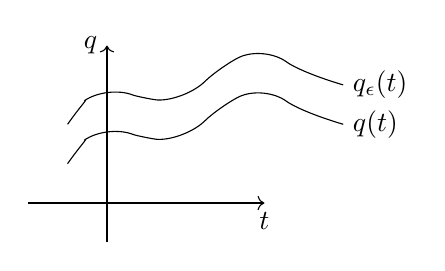
\begin{tikzpicture}[rounded corners = 10pt]
      \draw [->] (-1,0) -- (2,0) node [below] {$t$};
      \draw [->] (0,-.5) -- (0,2) node [left] {$q$};
      \draw (-.5,.5) to[bend left = 10] (0,1) to[bend right = 10] (1,.8)
        to[bend left = 10] (2,1.5) to[bend right = 10] (3,1)
        node [right] {$q(t)$};
      \draw [yshift = .5cm]
        (-.5,.5) to[bend left = 10] (0,1) to[bend right = 10]
        (1,.8)   to[bend left = 10] (2,1.5) to[bend right = 10] (3,1) node [right] {$q_\epsilon(t)$};
    \end{tikzpicture}
  \end{center}
\end{example}
\begin{example}[rotation]
  \[
    \bm q_\epsilon(t) = \bm q(t) + \epsilon \bm e_a \times q(t), \quad
    \bm f(t) = \bm e_a \times \bm q(t)
  \]
  The rotation of the world line.
  Figure: the world line rotate a angle between two time point real surface.
\end{example}
\begin{example}[time-translation]
  \[
    q_\epsilon(t) = q(t - \epsilon), \quad
    f(t) = -\dot q(t)
  \]
  \begin{center}
  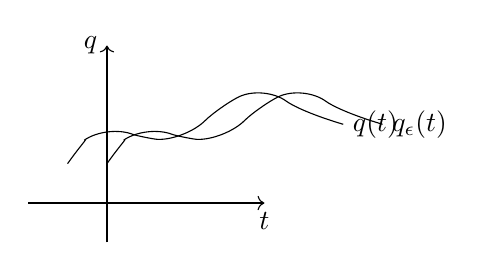
\begin{tikzpicture}[rounded corners = 10pt]
      \draw [->] (-1,0) -- (2,0) node [below] {$t$};
      \draw [->] (0,-.5) -- (0,2) node [left] {$q$};
      \draw (-.5,.5) to[bend left = 10] (0,1) to[bend right = 10] (1,.8)
        to[bend left = 10] (2,1.5) to[bend right = 10] (3,1)
        node [right] {$q(t)$};
      \draw [xshift = .5cm]
        (-.5,.5) to[bend left = 10] (0,1) to[bend right = 10]
        (1,.8)   to[bend left = 10] (2,1.5) to[bend right = 10] (3,1) node [right] {$q_\epsilon(t)$};
  \end{tikzpicture}
  \end{center}
\end{example}
For $t$-independent $\Omega_\theta$, the functional derivative
\begin{align*}
  0 & = \odv{\mathcal S[\Omega_\theta q]}\theta \bigg|_{\theta=0}
    = \frac1\epsilon (\mathcal S[\Omega_\epsilon q] - \mathcal S[q])
      \bigg|_{\epsilon \to 0}
    = \int_{t_i}^{t_f} \d t
      \ab(\pdv{\mathcal L}q \pdv{q_\theta}\theta
    + \pdv{\mathcal L}{\dot q} \pdv{\dot q_\theta}\theta) \\
    & = \int_{t_i}^{t_f} \d t
        \underbrace{\ab(\pdv{\mathcal L}q - \odv*{\pdv{\mathcal L}{\dot q}}t) f}
        _\text{E-L Equation}
      + \ab(\pdv{\mathcal L}{\dot q}f)\bigg|_{t_i}^{t_f}
\end{align*}
where we integral on shell, and
\[
  \mathcal S[q_\theta(t)] = \int_{t_i}^{t_f} \d t
  \mathcal L(q_\theta(t), \dot q_\theta(t), t)
\]
Since the E-L equation, we have
\[
  \ab(\pdv{\mathcal L}{\dot q}f)\bigg|_{t_i}^{t_f} = 0
\]
But $t_i$ and $t_f$ are arbitrary, so we can derive that
\[
  \odv*{\pdv{\mathcal L}{\dot q}f}t = 0
\]
means that it is independent from time, we get the conserved quantity.

So, in the first example $p$ is conserved; In the second one,
\[
  \mathcal S[q_\theta(t)] = \int_{t_i}^{t_f} \d t
  \mathcal L(\bm q_\theta(t), \dot{\bm q}_\theta(t), t)
\]
and
\[
  \ab(\sum_i \pdv{\mathcal L}{\dot q_i}f)\bigg|_{t_i}^{t_f} = 0
\]
so, $\bm e_a \cdot L = \bm p \cdot(\bm e_a \times \bm q(t))$
in the second example.

In the time-translation,
\[
  \mathcal S[q_\epsilon(t)] = \int_{t_i+\epsilon}^{t_f+\epsilon} \d t
  \mathcal L(q_\epsilon(t-\epsilon), \dot q_\epsilon(t-\epsilon), t)
\xlongequal{\tilde t = t - \epsilon} \int_{t_i}^{t_f} \d \tilde t
  \mathcal L(q(\tilde t), \dot q(\tilde t), \tilde + \epsilon)
\]
The derivative
\[
  0 = \odv{\mathcal S[\Omega_\theta q]}\theta \bigg|_{\theta=0}
    = \frac1\epsilon(\mathcal S[\Omega_\epsilon q] - \mathcal S[q])
    = \int_{t_i}^{t_f} \d t \pdv{\mathcal L}t \Rightarrow \pdv{\mathcal L}t = 0
\]
To interrupt it, we consider the total derivative
\[
  \odv*{\mathcal L}t = \pdv*{\mathcal L}q \dot q
+ \pdv*{\mathcal L}t\ab(\odv*{\dot q}t) + \pdv*{\mathcal L}t
\]
The second term
\[
  \pdv*{\mathcal L}t\ab(\odv*{\dot q}t)
= \odv*[fun]{\pdv{\mathcal L}q \dot q}t
- \ab(\odv*{\pdv{\mathcal L}{\dot q}}t)\dot q
\]
Substitute it and rearrange
\[
  0 = \pdv{\mathcal L}t = \odv*{\underbrace{\ab(
    \mathcal L - \pdv{\mathcal L}{\dot q} \dot q)}_\text{Hamiltonian}}t
- \underbrace{\ab(\pdv{\mathcal L}q - \odv*{\pdv{\mathcal L}q}t)}_
  \text{E-L equation} \dot q
\]
Then, we have the on-shell
\[
  \odv*{\mathcal H}t = 0
\]
i.e., the energy is conserved.

\paragraph{From (good) quantum numbers to group irrepresentation}

The statement is if
\[
  [\hat A, \hat B] = 0, \Rightarrow \exists \text{basis} \{\ket|\lambda>\}
\]
The basis vector is the eigenvector of both $\hat A$ and $\hat B$
\[
  \hat A\ket|\lambda> = \lambda_A\ket|\lambda>, \qq{and}
  \hat B\ket|\lambda> = \lambda_B\ket|\lambda>.
\]
\begin{proof}
  Consider $\hat A$ and $\hat B$ are Hermition.
  Take the ground state
  \[
    \hat A\ket|\alpha> = \alpha\ket|\alpha>
  \]
  In the case of degeneracy,
  \[
    \hat A\ket|\alpha_i> = \alpha\ket|\alpha_i>, \quad
    i = 1,\ \ldots\,,~d_\alpha
  \]
  Then, consider
  \[
    \hat A(\hat B\ket|\alpha>) = \hat B\hat A\ket|\alpha>
  = \alpha(\hat B\ket|\alpha>)
  \]
  means that
  \[
    \begin{cases*}
      \hat B\ket|\alpha> = b^{(\alpha)}\ket|\alpha>, & no-degeneracy\\
      \hat B\ket|\alpha_i> = \sum_j \ket|\alpha_j> b_{ji}^{(\alpha)}, &
      degeneracy
    \end{cases*}
  \]
  where $b_{ji}^{(\alpha)} = \braket<\alpha_j|\hat B|\alpha_i>$.
  We can always diagonalize
  \[
    b^{(\alpha_i)} = V D V^{-1}, \quad b^{(\alpha_i)} V = VD
  \]
  $D$ being a diagonal matrix $D_{ml} = \beta_l^{(\alpha)} \delta_{ml}$.
  Then,
  \[
    \sum_i b_{ji}^{(\alpha)} V_{il} = \sum_m V_{jm} D_{ml}
  = V_{jl} \beta_l^{(\alpha)}
  \]
  By take one superposition of the orginal $\alpha$
  \[
    \ket|\tilde \alpha_l> = \sum_i \ket|\alpha_i> V_{il}
  \]
  It is easy to know
  \[
    \hat B\ket|\tilde\alpha_\lambda> = \sum_i \hat B\ket|\alpha_i> V_{il}
  = \sum_{ij} \ket|\alpha_j>b_{ji}^{(\alpha)} V_{il}
  = \ket|\tilde\alpha_l> \beta_l^{(\alpha)}
  \]
  Then, the site
  \[
    \{\ket|\tilde\alpha_l>\} = \{\ket|\lambda>\}
  \]
  if there is no degeneracy, then $\ket|\tilde\alpha> = \ket|\alpha>$.
\end{proof}

\section{Symmetry group representations, degeneracies,
         inversion and time reversal}

\subsection{Group representations}

Starting from
\[
  \hat\Omega_\theta \ket|\bm r> = \ket|h_\theta(\bm r)>
\]
\begin{example}\leavevmode
  \begin{enumext}
    \item Translation $h_{\bm a} (\bm r) = \bm r + \bm r$
    \item Reflection $h_{\bm e}(\bm r) = \bm r - 2\bm r_\parallel$ (Figure required).
    \item Rotation $h_{\bm\theta = (\bm e_a, \theta)}(\bm r)
    = \bm r_\parallel + \cos\theta\bm r_\bot + \sin\theta(\bm e_a \times \bm r_\bot)$.
  \end{enumext}
  For an arbitary state $\ket|\psi>$, how the operator act on the arbitary state
  \[
    (\hat\Omega_\theta\psi)(\bm r)
  = \braket<\bm r|\hat\Omega_\theta|\psi>
  = \braket<h_\theta^{-1}(\bm r)|\psi> = \psi(h_\theta^{-1}(\bm r))
  \]
  Then, consider a general
  \[
    (\hat\Omega_2\hat\Omega_1\psi)(\bm r)
  = \braket<\bm r|\hat\Omega_2\hat\Omega_1|\psi>
  = \braket<h_2^{-1}(\bm r)|\Omega_1\psi>
  = \braket<(h^{-1}h_2^{-1})(\bm r)> \ket|\psi>
  \]
  where we can treat $\hat\Omega_2\hat\Omega_1 = \hat\Omega_3$.
  The transformation converses the distance $\bm r_1 - \bm r_2$,
  then, all the $h$
  \[
    h(\bm r_1 - \bm r_1) = |h(\bm r_1) - h(\bm r_1)| = |\bm r_1 - \bm r_2|
  \]
  form the Euclidian space (Group)
  \begin{equation}
    E(d):\ \{h||h(\bm r_1 - \bm r_2) = |\bm r_1 - \bm r_2|\}
  \end{equation}
  \begin{enumext}
    \item All the translation form $T(d)$
    \item All the reflection form $O \in \text{reflection place}$
    \item All the rotationform $O(d)$, orthogonal group.
  \end{enumext}
  But, in Euclidian space, it will become a semi-direct product
  \[
    T_d \rtimes O(d)
  \]
  where $O(d) = \text{SO}(d) \times \mathbb Z_2$ is orthogonal.
  For $\{M_d:\ M^\dagger M = \identity\}$, then $(\det(M))^2 = 1$,
  $\det(M) = \pm 1$. This means that $S$ can be special for $\det(M) = +1$.
  While $Z_2$ have two $\{+1, -1\}$.
\end{example}

We have a Euclidian group
$\{\hat\Omega_\theta\} \leftarrow G = E(d) \to \{h_\theta\}$ corresponding to
all the operators.
\begin{equation}
  \overset{\mathbb V = \{\ket|\bm r>\}}
    {\underset{(G\circlearrowright\mathbb V)}{\{\hat\Omega_\theta\}}}
  \xlongleftarrow[\substack{
    \Omega_1\mapsfrom g_1,\ \Omega_2\mapsfrom g_2\\
    \Omega_1\Omega_2 \mapsfrom g_1 \cdot g_2
  }]{\text{homomorphism}}
  \underset{\substack{\rotatebox{90}{$=$}\\E(d)}}{G}
  \xlongrightarrow{\text{homo}}
  \overset{\mathbb R = \{\bm r\}}
    {\underset{(G\circlearrowright\mathbb R^d)}{\{\hat h_\theta\}}}, \quad
  G \longrightarrow GL(V), \quad \Omega: V \to V
\end{equation}
where ``homomorphism'' means the same shape and form,
$h_\theta$ acts on $\bm r$ while $\hat\Omega_\theta$ acts on $\ket|\bm r>$.
They form \emph{Group Action}: Representation.

\paragraph{Translation group}

We start from the translation group $T(d)$. Consider
\[
  T_{\bm a} \cdot T_{\bm b} = T_{\bm a + \bm b = \bm b + \bm a}
\]
we call it the \emph{Abelian Group}.
In Hilbert space of this case, $V = \operatorname{span}(\{\ket|\bm r>\})$.
Then, the operator $\hat T_{\bm a}$ on this space
\[
  \hat T_{\bm a} = \upe^{-\iu\bm a\cdot\hat{\bm k}}
\]
where $\hat g_{T_i} = \hat k_i$ for $i = 1$, $2$, $3$.
\paragraph{Quiz}
Now, consider
\[
  T_{\bm a} \xlongequal{k\to\iu\nabla} \upe^{-\bm a \cdot\nabla}
\]
Calculate
\[
  \braket<\bm r|\hat T_a|\psi> = (T_{\bm a}\psi)(\bm r)
= \psi(\bm r - \bm a).
\]
By Foruier transform , where one can have the eigenvalue Equation
\[
  \nabla \upe^{\iu\bm k\cdot\bm r} = -\iu \bm k \upe
\]
and in Foruier transform
\[
  \psi(\bm r) = \int \d\bm k \tilde\psi(\bm k) \upe^{\iu\bm k\cdot\bm r}
\]
we can have
\[
  f(\nabla) \upe^{\iu \bm k\cdot\bm r} = f(\iu\bm k) \upe^{\iu\bm k\cdot\bm r},
  \quad
  \upe^{-\bm a\cdot\nabla} \upe^{\iu\bm k\cdot\bm r}
= \upe^{\iu\bm k\cdot(\bm r-\bm a)}
\]
Due to the property of the transform operator
\[
  \upe^{-\bm a\cdot\nabla} \psi(\bm r) = \psi(\bm r - \bm a)
\]
substitute the identities above
\[
  \upe^{-\bm a\cdot\nabla} \psi(\bm r)
= \int \d\bm k \tilde\psi(\bm k) \upe^{\iu\bm k(\bm r-\bm a)}
= \psi(\bm r - \bm a)
\]
\rule{\linewidth}{1pt}
For Abelian group, we have the commutative generator
\[
  [\hat k_i, \hat k_j] = 0
\]
\begin{enumext}
  \item $V = \{\ket|\bm k, \sigma>|\hat{\bm k} \ket|\bm k,
    \sigma> = \bm k\ket|\bm k, \sigma>, \bm k \in \mathbb R^3\}$.
  Now, the Hilbert space becomes a direct sum
  \[
    V = \bigoplus_{\bm k\in\mathbb R^3} V_{\bm k}, \qq{where}
    V_{\bm k_0} = \operatorname{span}(\{\ket|\bm k_\sigma, \sigma>\})
  \]
  \item $[\hat H, \hat{\bm k}] = 0$, $\forall \bm a$. The Hamiltonian operator
  also becomes
  \[
    \hat H = \bigoplus_{\bm k\in\mathbb R^3} \hat H_{\bm k}
  = \pdiagmat[empty = {}]{H_{\bm k_1}, H_{\bm k_2}, \ddots}
  \]
  where
  \[
    \hat H_{\bm k} = P_{\bm k} \hat H P_{\bm k}, \qq{and}
    P_{\bm k} = \sum_\sigma \ketbra|\bm k,\sigma><\bm k, \sigma|
  \]
  Then, $V_{\bm k} = P_{\bm k}V$, the so-called \emph{Bloch Theorem}\footnote{%
    In the lattice, we need to change $\bm a \in \mathbb R^3 \to \mathbb Z^3$}.
\end{enumext}

\paragraph{Non-abelian Group}

\begin{example}
  $\text{SO}(d)$ for $d > 2$
\end{example}
\begin{example}[Dihedred Group for $n$-gon]
  The elements
  \[
    \{e,\ R,\ R^2, \rho_0, \rho_1,\ \rho_2\} = \bra<R,\rho = \rho_0|
    \qq{(generators)}
  \]
  where
  \begin{enumext}[columns = 2]
    \item $R^2 = \bar R$
    \item $\rho_i = \bar\rho_i$
    \item $R^3 = e = \rho_i$
    \item $R\rho_i\bar R = \rho_{i+1}$
    \item $\rho R \bar\rho_0 = \bar R$
  \end{enumext}
  In summary
  \begin{enumext}[columns = 2]
    \item $R\rho_0\bar R = \rho_{R(0)}$
    \item $\rho_0 R\bar\rho_0 = R_\text{flip} = \bar R$
    \item $\rho_i\rho_{i+1} = R$
    \item $\rho_{i+1}\rho_i = \bar R$
  \end{enumext}
  From $\rho_a\rho_b = T_{2(a+b)}$, we have
  \[
    \rho_i \rho_{i\pm 1} = T_{\mp2} = T_{\pm 1} = R^2
  \]
  and from $\rho_a\rho_b\rho_c = \rho_{a-b+c}$, we have
  \[
    \rho_0\rho_1\bar\rho_0 = \rho_{0-1+0} = \rho_{-1} = \rho_2
  \]
  \[
    R\rho_0 = \rho_2 \rho_0 \rho_0 = \rho_2, \quad
    R^2 \rho_0 = \rho_1
  \]
\end{example}
Cayley Table (Group Multiplication Table)
\[
  \{e,\ R,\ R^2, \rho_0, \rho_1,\ \rho_2\} = \braket<\underbrace{R,\rho = \rho_0}_\text{generators}|
  \underbrace{R^3 = \rho^2 = e, \rho R = R^2\rho}_\text{relations}>
\]
where $R^{n_1}$, $\rho^{m_1}$, $R^{n_2}$, $\rho_{m_2}$
will appear in the group. We can always switch $R$ and $\rho$ since
\[
  \rho R = R^2 \rho
\]
Similar for $D_n$.

Now, we can define two operators
\[
  \hat R\ket|i> = \ket|R(i)> = \ket|i + 1>, \qq{and}
  \hat\rho\ket|i> = \ket|\rho(i)> = \ket|-i>
\]
on Hilbert space $V = \operatorname{span}(\{\ket|0>, \ket|1>, \ket|2>\})$.
The Hamiltonian
\[
  \hat H = \sum_{i,j = 0,1,2} \ketbra|i> h_{ij} <j|
\]
where $h_{ij} = h_{ji}^*$. So,
\[
  \forall \hat g \in D_3,\ [\hat H, \hat g] = 0 \Rightarrow ?
\]
Since $\hat R\hat H\hat R^{-1} = \sum_{ij} \ketbra|i+1>h_{ij}<j+1| = \hat H$, then
\[
  h_{ij} = h_{i+1,j+1}, \quad
  h_{ij} = h_{-i, -j}
\]
we have
\[
  \hat H = \begin{pmatrix}
    \epsilon & t & t\\ t& \epsilon & t\\t & t' & \epsilon
  \end{pmatrix} =
  \begin{pmatrix}
    0 & t  & t\\
    t & 0  & t\\
    t & t' & 0
  \end{pmatrix}
\]
The eigenvalue and eigenvector, the basis are $\ket|0>$, $\ket|1>$, $\ket|2>$.
\[
  \hat H = t(\hat R + \hat R^2)
\]
we know $\hat R^3 = 1$, then the eigenvalue should be
$\lambda_n = \upe^{\iu\frac{2\pi}3}$
\[
  \hat R\ket|\psi_n> = \upe^{\iu\frac{2\pi}{3}n} \ket|\psi_n>, \quad
  n = 0,\ 1,\ 2
\]
Then eigenvalues are
\[
  E_{\psi_0} = 2t, \quad E_{\psi_1} = E_{\psi_2} = t(\omega + \omega^*)
\]
we arrive at the degeneracy.
Now, write the operators $\hat R$ and $\hat \rho$ into the basis
\[
  \{\ket|\psi_0>,\ \ket|\psi_1>,\ \ket|\psi_2>\}
\]
$R_\psi$ in the $\psi$ basis, it is diagonal
\[
  R_\psi = \pdiagmat{1, \omega, \bar\omega}
\]
Calculate how $\hat R(\hat\rho\ket|\psi_0>)$ acts.
\[
  \hat R(\hat\rho\ket|\psi_0>) = \hat\rho \hat R^2 \ket|\psi_0>
\xlongequal{\hat R\ket|\psi_0> = \ket|\psi_0>} \hat\rho\ket|\psi_0>
\]
So, $\braket<\psi_i|\hat\rho|\psi_0> = \delta_{i,0}$.
For $\ket|\psi_1>$,
\[
  \hat R(\hat\rho\ket|\psi_1>) = \hat\rho \hat R^2 \ket|\psi_1>
= \bar\omega \hat\rho \ket|\psi_1>
\]
So, in matrix
\[
  R_\psi = \begin{pmatrix}
    1 & & 0\\
    & \omega\\
    0 & & \bar\omega
  \end{pmatrix}, \quad
  \rho_\psi = \begin{pmatrix}
    1 & 0\\
    0 & & 1\\
    & 1
  \end{pmatrix}
\]
In the new basis, the Hilbert space
\[
  V = V_{\psi_0} \oplus V_{\{\psi_1, \psi_2\}}, \quad
  g = g_{\psi_0} \oplus g_{\{\psi_1,\psi_2\}}
\]
and
\[
  0 = \braket<\psi_1|\hat\rho|\psi_1>
\]
This is why the degeneracy occurs.
\[
  \hat H\ket|\psi> = E\ket|\psi>, \quad
  \hat H(\hat\rho\ket|\psi>) = \hat\rho \hat H\ket|\psi>
= E(\hat\rho\ket|\psi>).
\]

\paragraph{Quick Review of Group Representation}

Starting from
\[
  \underset{\text{Group}}G
  \overset{\tau}{\underset{\text{acts on}}{\circlearrowright}}
  \underset{\text{linear space}}V, \quad
  \tau:\ G \rightarrow
  \underset{\text{Linear operator space on $V$}}
    {\overset{\text{opened}}G\overset{\text{linear}}L(V)}
\]
where $\tau$ is homomorphism:
\[
  \forall \underset{\rotatebox{-90}{$\mapsto A_{1,2}$}}{g_{1,2}} \in G, \quad
  (g_1 \circ g_2) \longmapsto A_1 A_2
\]

\begin{example}
  For the group $D_3 = \{e, R, R^2, \rho_0, \rho_1, \rho_2\} \cong S_3$
  which satisfy $R^3 = \rho^2 = e,\ R\rho = \rho R^2$.
  \begin{paracol}{2}
    \[
      (\quad),\ (012) = (120) = (201),\ (021),\ (12),\ (20),\ (01)
    \]
    For example, $(12)(12) = (\quad)$, $(012)(12) = (10)$.
    \switchcolumn \centering
    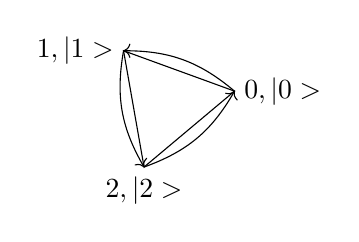
\begin{tikzpicture}[scale = 1.5]
      \draw [rotate = 10] (0,0) coordinate (a)
       node [left] {$1, \ket|1>$} -- (0,-1) coordinate (b)
       node [below] {$2, \ket|2>$} -- ({sqrt(3)/2},-.5)
       coordinate (c) node [right] {$0, \ket|0>$} -- cycle;
      \draw [->] (c) to[bend right = 20] (a);
      \draw [->] (a) to[bend right = 20] (b);
      \draw [->] (b) to[bend right = 20] (c);
    \end{tikzpicture}
  \end{paracol}
  Then, for the group multiplication
  \[
    (12)(012) = (12)(120) = (12)(12)(20) = (20), \quad
    (12)(021) = (12)(210) = (12)(21)(10) = (10)
  \]
  Consider taking $i \mapsto \ket|i>$, basis of Hilbert space $V$
  ($\{\ket|0>, \ket|1>, \ket|2>\}$). Then, the identities become
  \[
    \hat R\ket|i> = \ket|R(i)>,   \quad
    \hat R\rho\ket|i> = \ket|\rho(i)>.
  \]
  Then, we can say $\{e, R, R^2, \rho_0, \rho_1, \rho_2\} \subset V$.
  The Hilbert space can be composed into two parts
  \[
    V = V_{\psi_0} \oplus V_{\{\psi_1,\psi_2\}}
  \]
  where $\ket|\psi_n>$ means $\hat R\ket|\psi_n> = \omega^n \ket|\psi_n>$,
  $\omega = \upe^{\iu\frac{2\pi}{3}}$.
  So, the subspace
  \[
    V_{\psi_0} = \operatorname{span}(\{\psi_0\}),\
    V_{\{\psi_1,\psi_2\}} = \operatorname{span}(\{\psi_1,\psi_2\})
  \]
  $\forall \hat g \in \hat D_3$,
  \[
    g =
    \begin{pNiceArray}{c|cc}[first-col, last-row]
      \ket|\psi_0> &
      \Block[tikz = {pattern = north east lines, pattern color = teal}]{}{}
      & \Block{1-2}{O}\\
      \hline
      \ket|\psi_1> & \Block{2-1}{O} &
      \Block[tikz = {pattern = north east lines, pattern color = teal}]{2-2}{}\\
      \ket|\psi_2> & \\
    & \bra<\psi_0| & \bra<\psi_1| & \bra<\psi_2|
    \end{pNiceArray}
  \]
  where the generator
  \[
    R = \begin{pNiceArray}{c|cc}
      1 & \Block{1-2}{O}\\
      \hline
      \Block{2-1}{O} & \omega\\
      & & \omega^*
    \end{pNiceArray}, \quad
    \rho = \begin{pNiceArray}{c|cc}
      1 & \Block{1-2}{O}\\
      \hline
      \Block{2-1}{O} & & 1\\
      & 1
    \end{pNiceArray}
  \]
  we label the subspace $V_{\psi_0}$ as $A_1$, and label $V_{\{\psi_1,\psi_2\}}$
  as $E$. Then
  \[
    e_A = 1,\quad R_{A_1} = 1, \quad \rho_{A_1} = 1 \Rightarrow g_{A_1} = 1,
  \]
  \[
    e_E = \pdiagmat[empty = {}]{1,1},\quad
    R_E = \pdiagmat[empty = {}]{\omega, \omega^*}, \quad
    \rho_E = \begin{pmatrix}
      & 1\\1
    \end{pmatrix} \text{(Equivalent Representations)}
  \]
  The multiplication
  \[
    R_E \rho_E = \begin{pmatrix}
      0 & \omega \\ \omega^* & 0
    \end{pmatrix} = \rho_E R_E^2 = \begin{pmatrix}
      & \omega \\\omega^*
    \end{pmatrix} \pdiagmat[empty = {}]{\omega^*, \omega}.
  \]
  For non-Abelian group, $\hat R\hat \rho \neq \hat \rho \hat R$.
  \[
    \text{\underline{minimal} invariant subspace} \leftrightarrow
    \text{\underline{irreducible} (sub)representation}
  \]
\end{example}
Now, consider the Hilbert space becomes
\[
  \operatorname{opan}(\{\ket|0\pm>, \ket|1\pm>, \ket|2\pm>\}).
\]
Induce
\[
  i \pm \mapsto \ket|i\pm>, \quad
  \hat R\ket|i,s> = \ket|i+1,s>,\
  \hat\rho \ket|i,s> = \ket|-i,-s>
\]
Consider the Hamiltonian
\[
  \hat H = \sum_{j,s,j',s'} \ketbra|j,s>h_{js;j's'} <j's'|
\]
which satisfies
\[
  [\hat R, \hat H] = [\hat\rho, \hat H] = 0
\]
\[
  \begin{array}{c}
    \{\text{Transformations on Real Space}\}\\
    \text{def} \downarrow \uparrow \text{represent}\\
    G\\
    \downarrow \text{represent}\\
    \{\text{Transformations on
      $\underset{\text{HS $V$ represent}
        \{\text{Transformations on Operator Space}\}}
        {\text{Function Space}}$}\}, \quad \{V \to V\}
  \end{array}
\]
For invariant subspace $W$ (group action):
$\forall g \in G$, $\ket|w> \in W$, we have
\[
  \hat g (= \tau(g)) \ket|w> \in W
\]
Now, minimal invariant subspace $\leftrightarrow$ irreducible representation.
Choose $\ket|\psi_1>$, which satisfies
\[
  \hat H\ket|\psi_1> = E\ket|\psi_1>
\]
Then, $\ket|\psi_2> = \hat\rho\ket|\psi_1>$, and they are orthogonal to each
other $\braket<\psi_2|\psi_1> = 0$, then
\[
  \hat H \hat \rho \ket|\psi_1> = E\hat \rho \ket|\psi_1>
\]
\paragraph{Schur's Lemma}
In irrepresentation $\tau$, if $[\hat H_\tau, \hat g_\tau] = 0$
$\forall g \in G$, then it is the irrepresentation of $G$.
Then, $\hat H_\tau = E\identity_\tau$,
which call $\dim(V_\tau) = \#\text{Degeneracy}$.

\paragraph{Space Inversion \& Time Reversal}

\begin{center}
  \begin{minipage}[t]{.64\linewidth}
    \centering
    \begin{tabular}{*3l}
      \toprule
      Classical & $\mathcal I = \rho_x \rho_y \rho_z$ & $\mathcal T$\\
      \midrule
      & $\bm r \to -\bm r$, $t \to t$ &
      $t \to -t$, $\bm r \to \bm r$\\
      & $\bm p \to -\bm p$ & $\bm p \to -\bm p$\\
      \midrule
      Polar (Vector) & $\bm E \to -\bm E$ & $\bm E \to \bm E$\\
      Axial (Pseudo vector) & $\bm B \to \bm B$ & $\bm B \to -\bm B$\\
      $\bm E = -\nabla\varphi$ & $\varphi \to \varphi$ & $\varphi \to \varphi$\\
      $\bm A = \nabla \times \bm B$ & $\bm A \to -\bm A$ & $\bm A \to \bm A$\\
      \bottomrule
    \end{tabular}
  \end{minipage} \hfill
  \begin{minipage}[t]{.32\linewidth}
  Quantum:

  \begin{tabular}{ll}
    \toprule
    $\hat I$ & $\hat T$\\
    \midrule
    $\hat I \hat{\bm r} \hat I^{-1} = -\hat{\bm r}$ &
    $\hat T\hat{\bm r}\hat T^{-1} = \hat{\bm r}$\\
    $\hat I \hat{\bm p} \hat I^{-1} = -\hat{\bm p}$ &
    $\hat T\hat{\bm p}\hat T^{-1} = -\hat{\bm p}$\\
    $\hat I[\hat x, \hat p_x]\hat I^{-1} = [-\hat x, -\hat p_x] = \iu$ &
    $\hat T[\hat x, \hat p_x]\hat T^{-1} = [\hat x, -\hat p_x] = -\iu$\\
    \bottomrule
  \end{tabular}
  \end{minipage}
\end{center}

For $\hat f$ anti-linear
\[
  \hat f(a\ket|\psi> + b\ket|\chi>
= a^*\hat f\ket|\varphi> + b^*\hat f\ket|\chi>)
\]
Norm-preserving
\[
  \braket<\hat f\psi|\hat f\psi> = \braket<\psi|\psi>
\]
\paragraph{Quiz}
Prove that $\forall \psi,\ x_i$,
$\braket<\hat f\psi|\hat f\chi> = \braket<x|\psi> = \braket<\psi|\chi>^*$.
BTW, when it is satisfied, $f$ is called anti-unitary.

We already have
for $\hat I$: $\{e, I\}$, $I^2 = e$;
and for $T$: $\{e,T\}$, $T^2 = e$.
Combine irreps of $\{e,i\}$, and $i^2 = e$ called involution.
\[
  \ket|\psi> \sim \upe^{\iu\theta}\ket|\psi> \in V,
\]
then
\[
  \hat e\ket|\psi> = \ket|\psi>, \quad
  \hat i\ket|\psi> = \ket|\chi>, \quad
  \hat i^2 \ket|\psi> = \hat i \ket|\chi> = \upe^{\iu\theta} \ket|\psi>.
\]
Take $\ket|\chi> \propto \ket|\psi>$, then $\braket<\psi|\chi> = 0$.
Start with $\hat i$ be unitary with $\hat I$ is unitary.
We can always construct another state with a linear combination
\[
  \ket|\phi> = a\ket|\psi> + b\ket|\chi>,
\]
Then,
\[
  \ket|\phi> \propto \hat i_\pm\ket|\phi> = a_\pm\ket|\chi> + b\upe^{\iu\theta}\ket|\psi>
\]
Rearrange it
\[
  \frac{b\upe^{\iu\theta}}{a} = \frac ab, \quad
  \ab(\frac ab)^2 = \upe^{\iu\theta}, \quad
  g = 1,\ a_\pm = \pm \upe^{\iu\theta}
\]
For anti-unitary, we need to
\[
  \ket|\phi> \propto \hat i\ket|\phi>
= a^*\ket|\chi> + b^*\upe^{\iu\theta}\ket|\psi>
\]
Rearrange it
\[
  \frac{b^* \upe^{\iu\theta}}{a} = \frac{a^*}{b} \Rightarrow
  |a|^2 = |b|^2\upe^{\iu\theta}
\]
If $|a|^2 = |b|^2$, $\upe^{\iu\theta} = 1$.


\subsection{Degeneracies}

\section{Angular momentum, Lie algebra}

\section{Gauge}


\newcommand \sectionname {Lecture \#}
\appendix
\sidefoot \thepage
\fancyhead[OL, ER]{Mingyu Xia (Westlake ID: 20251202247)}
\fancyhead[EL]{\sffamily \rightmark}
\fancyhead[OR]{\fontfamily{lmr}\selectfont<<\texttt{\href{mailto:xiamingyu@westlake.edu.cn}{xiamingyu@westlake.edu.cn}}>>}
\addcontentsline{toc}{chapter}{Problem Set}
\renewcommand *\thesection{\sectionname \arabic{section}}
\newweek
% !TeX root = ../main.tex

\section{Review}

\begin{problem}
  Solve the Schr\"odinger equation (i.e., find the eigenvalues and eigenstates, then plot typical eigenstates) with the following 1D Hamiltonians
  \[\mathcal H = \frac{\hat p^2}{2m} + V(x),\]
  where
  \begin{enumext*}[columns = 7]
    \item(2) $V(x) = \frac12 m \omega^2 x^2$; (25')
    \item(5) $V(x) = V_0 \delta(L/2 - |x|)$ with $\delta(x)$
    the Heavisine step function; (15')
    \item(7) $V(x) = V_0 [\delta(x + L/2) + \delta(x - L/2)]$ with $\delta(x)$
    the Dirac delta function. (15')
  \end{enumext*}
\end{problem}
\begin{solution}\leavevmode
  \begin{enumext}
    \item Under this potential, the system appears as a Harmonic oscillator.
    Substitute the Hamiltonian into the time-independent Schr\"odinger equation
    \[
      \ab(-\frac{\hbar^2}{2m} \odv*[2]{}x + \frac12 m \omega^2 x^2) \psi(x)
    = E \psi(x).
    \]
    where $\hat p = -\iu\hbar \odv*{}x$. We define
    \begin{enumext}[columns = 4]
      \item $\alpha = \sqrt{m\omega / \hbar}$
      \item $\xi = \alpha x$, $x = \xi/\alpha$
      \item $\psi(x) = u(\xi)$
      \item $\lambda = 2E/\hbar\omega$
    \end{enumext}
    for simplification. Consider the asymptotic behavior of this ODE first
    \[
      \odv[2]{u(\xi)}{\xi^2} + (\lambda - \xi^2) u(\xi) = 0
      \xLongrightarrow{|\xi| \to \infty}
      \odv[2]{u(\xi)}{\xi^2} - \xi^2 u(\xi) = 0,
    \]
    and its asymptotic solution is $u(\xi) = \upe^{-\xi^2/2}$
    (Since $\upe^{+\xi^2/2}$ blows up, so it is discarded).
    Now, insert a polynomial $H(\xi)$ to obtain its solution in common solution
    \[
      u(\xi) = H(\xi) \upe^{-\xi^2/2},
    \]
    then substitute it into the ODE, and simplify it
    \[
      H'' - 2\xi H' + (\lambda - 1) H = 0.
    \]
    It is so-called \emph{Hermit Polynomial}.
    We assume the expansion of $H(\xi)$ is a power series
    \[
      H(\xi) = \sum_{n=0}^\infty a_n \xi^n,
    \]
    and then substitute it into the ODE
    \[
      \sum_{n=2}^\infty a_n n (n - 1) \xi^{n-2}
    - 2\xi \sum_{n=1}^\infty a_n n \xi^{n-1}
    + (\lambda - 1) \sum_{n=0}^\infty a_n \xi^n = 0.
    \]
    We have to combine the three sum terms.
    Since in the 2nd derivation of $H(\xi)$ the top 2 terms disappers,
    while in the 1st derivation of $H(\xi)$, the first term disappers,
    so the expansion can be
    \[
      \sum_{n=0}^\infty a_{n+2} (n + 2) (n + 1) \xi^n
  - 2 \sum_{n=0}^\infty a_n n \xi^n
  + (\lambda - 1) \sum_{n=0}^\infty a_n \xi^n = 0.
    \]
    \newpage
    Since there is a term contains single ``$n$'',
    so we need to discuss respectively.
    \begin{enumext}
      \item For $n = 0$, we have
      $2a_2 + \lambda - 1 = 0, \qq{and} a_2 = -(1 - \lambda)a_0/2$
      \item For $n \geq 1$, we have
      $a_{n+2} = [2n - (\lambda - 1)]/[(n + 2) (n + 1)] a_n$.
    \end{enumext}
    Apply \emph{d'Alembert's Judgement} to the $n$th
    and the $n + 2$th terms of $H(\xi)$
    \[
      \lim_{n\to\infty} \frac{a_{n+2} \xi^{n+2}}{a_n \xi^n}
    = \lim_{n\to\infty} \frac{2n - (\lambda - 1)}{(n + 2) (n + 1)} \xi^2
  \sim\frac2n \xi^2,
    \]
    means that $H(\xi)$ will divergent.
    To avoid this,
    the series needs to be cut off at $n$th term ($n$ is finite), let
    \[
      a_{n+2} = [2n - (\lambda - 1)]a_n/[(n + 2) (n + 1)] = 0,
    \]
    since $a_n \neq 0$, so $2n - (\lambda - 1) = 0$, that is
    \[
      \lambda = 2n + 1 = 2E/\hbar\omega, \qq{and}
      E = \hbar \omega (n + 1/2).
    \]
    From the limitation of wave function,
    we arrive at the discrete energy level.
    Now, normalize it
    \[
      \braket<\psi(x)|\psi(x)>
    = \int_{\mathbb R} [H_n(\xi)]^2 \upe^{-\si^2} \d \xi/\alpha = 1,
    \]
    using the orthogonality property of Hermit polynomial
    \[
      \int_{\mathbb R} H_m(\xi) H_n(\xi) \upe^{-\xi^2} \d \xi
    = \sqrt\pi 2^n n! \delta_{mn},
    \]
    we arrive at the normalized wave function
    \[
      \psi_n(x) = \frac1{\sqrt{2^nn!}} \ab(\frac{m\omega}{\pi\hbar})^{1/4}
      H_n\ab(\sqrt{\frac{m\omega}{\hbar}}x)
      \exp\ab(-\frac{m\omega}{2\hbar}x^2),
      \qq{or}
      \psi_n(\xi) = \sqrt{\frac{\alpha}{\sqrt\pi 2^n n!}}
      H_n(\xi) \upe^{-\xi^2/2}.
    \]
    For the typical state:
    \begin{enumext}
      \item $\psi_0(x) = \sqrt{\frac{\alpha}{\sqrt\pi}}
        \upe^{-\alpha^2x^2/2}$, is a Gaussian distribution.
      \item $\psi_1(x) = \sqrt{\frac{\alpha}{2\sqrt\pi}}
        (2 \alpha x) \upe^{-\alpha^2x^2/2}$, is odd.
      \item $\psi_2(x) = \sqrt{\frac{\alpha}{8\sqrt\pi}}
        (4 \alpha^2 x^2 - 2) \upe^{-\alpha^2x^2/2}$, is even.
    \end{enumext}
    The figures of the typical eigenstates:
    Ground state ($n = 0$), first excited state ($n = 1$), and
    second excited state ($n = 2$) plotted by \textsf{MATLAB}
    are listed as follows
    \begin{figure}[H]
      \begin{subfigure}{.32\linewidth}
        \centering
        \includegraphics[width = .98\linewidth, page = 1]{./media/hw0_fig1}
        \caption{Ground state $\psi_0(x)$}
      \end{subfigure}
      \hspace*\fill
      \begin{subfigure}{.32\linewidth}
        \centering
        \includegraphics[width = .98\linewidth, page = 2]{./media/hw0_fig1}
        \caption{1st excited state $\psi_1(x)$}
      \end{subfigure}
      \hspace*\fill
      \begin{subfigure}{.32\linewidth}
        \centering
        \includegraphics[width = .98\linewidth, page = 3]{./media/hw0_fig1}
        \caption{2nd excited state $\psi_2(x)$}
      \end{subfigure}
    \end{figure}

    The \textsf{MATLAB} source code for the three eigenstates
    is also attached as follows.
    \inputminted[obeytabs, linenos, framesep = 3pt] {matlab}
      {./media/hw0_fig1.m}
    \item Under this potential, the system appears as a potential barrier
    and can be divided into three regions:
    \begin{enumext}
      \item Region I and III ($|x| > L/2$):
      the wave function decays exponentially.
      \item Region II ($|x| \leq L/2$):
      the wave function behaves oscillatory.
    \end{enumext}
    The Hamiltonian is
    \[
      \mathcal H = \frac{\hat p^2}{2m} + V_0 \delta(L/2 - |x|),
    \]
    where $\hat p = -\iu\hbar \odv*{}x$.
    The Schr\"odinger equation for the system is
    \begin{alignat*}{2}
      -\frac{\hbar^2}{2m} \odv*[2]{}x \psi(x)               & = E \psi(x), \quad
      & \text{Region I and III}\\
      \ab(-\frac{\hbar^2}{2m} \odv*[2]{}x + V_0) \psi(x)    & = E \psi(x), \quad
      & \text{Region II}
    \end{alignat*}
    \begin{enumext}[wrap-label = \underline{Case #1}, label = \arabic*,
                    list-indent = 0pt]
      \item Energy above the barrier ($E > V_0$)\\
      Define
      \[
        k = \sqrt{\frac{2mE}{\hbar^2}}, \qq{and}
        \kappa = \sqrt{\frac{2m(E - V_0)}{\hbar^2}},
      \]
      the Schr\"odinger equation becomes
      \begin{align*}
        & \psi''(x) + k^2 \psi(x)      = 0, &&
        \text{Regions I and III}\\
        & \psi''(x) + \kappa^2 \psi(x) = 0, && \text{Regions II}\\
      \intertext{and its the solution in the three regions is}
        & \psi_\text I(x)    = \upe^{\iu k x} + r \upe^{-\iu kx},
        && \text{Region I: Incident \& reflected waves}\\
        & \psi_\text{III}(x) = t \upe^{\iu kx},
        && \text{Region III: Transmitted wave}\\
        & \psi_\text{II}(x)  = C \upe^{\iu\kappa x} + D \upe^{-\iu\kappa x},
        && \text{Region II: Transmitted \& reflected wave inside the barrier}
      \end{align*}
      To find the eigenstates, apply the boundary conditions at $x = \pm L/2$,
      that is
      \[
        \psi_\text I^{(0,1)}(-L/2)   = \psi_\text{II}^{(0,1)}(-L/2), \qq{and}
        \psi_\text{III}^{(0,1)}(L/2) = \psi_\text{II}^{(0,1)}(L/2).
      \]
      We get a Quaternion linear equation system. By canceling $C$ and $D$,
      we derived the transmission coefficient $T = |t|^2$
      and reflection coefficient $R = |r|^2$
      \[
        T = \frac{4k^2 \kappa^2 \cos^2(\kappa L)}
        {(k^2 - \kappa^2)^2 \sin^2(\kappa L) + 4k^2 \kappa^2 \cos^2(\kappa L)},
        \qq{and}
        R = \frac{(k^2 - \kappa^2)^2 \sin^2(\kappa L)}
        {(k^2 - \kappa^2)^2 \sin^2(\kappa L) + 4k^2 \kappa^2 \cos^2(\kappa L)}.
      \]
      \item Energy below the Barrier ($E_0 < V_0$)\\
      This case can be considered as $\kappa \to \iu \kappa$.
      Reusing the conclusion from case $E > V_0$, the wave function
      \[
        \psi_\text I(x)     = \upe^{\iu kx} + r \upe^{-\iu kx},~
        \psi_\text{III}(x)  = t \upe^{\iu kx},~
        \psi_\text{II}(x)   = C \upe^{-\kappa x} + D \upe^{\kappa x},
      \]
      and the transmission \& reflection coefficient
      \[
        T = \frac{4k^2 \kappa^2 \cosh^2(\kappa L)}
          {(k^2 + \kappa^2)^2 \sinh^2(\kappa L) + 4k^2 \kappa^2 \cosh^2(\kappa L)},
        \qq{and}
        R = \frac{(k^2 + \kappa^2)^2 \sinh^2(\kappa L)}
        {(k^2 + \kappa^2)^2 \sinh^2(\kappa L) + 4k^2 \kappa^2 \cosh^2(\kappa L)}.
      \]
      here used the identities for hyperbolic functions:
      $\sin(\iu x) = -\iu \sinh(x)$, $\cos(\iu x) = \cosh(x)$.
      \item Energy equal to the barrier ($E = V_0$)\\
      Now, $\kappa = 0$. So, in Region II
      \[
        \psi''(x) = 0, \quad \psi_\text{II}(x) = Cx + D,
      \]
      while the expression of the wave function in Region I and Region III
      remains unchanged. Concerning the transmission \& reflection coefficient,
      we can calculate the limitation directly
      \[
        \lim_{\kappa\to0} T = \frac{4}{4 + (kL)^2}, \qq{and}
        \lim_{\kappa\to0} R = \frac{(kL)^2}{4 + (kL)^2}.
      \]
    \end{enumext}
    The figures of the typical eigenstates:
    Propagation wave function ($E > V_0$), Tunneling wave function ($E < V_0$),
    and the Critical Wave Function ($E = V_0$)
    are plotted by \textsf{MATLAB} and listed as follows
    \begin{figure}[H]
      \begin{subfigure}{.32\linewidth}
        \centering
        \includegraphics[width = .98\linewidth, page = 1]{./media/hw0_fig2}
        \caption{$E > V_0$}
      \end{subfigure}
      \hspace*\fill
      \begin{subfigure}{.32\linewidth}
        \centering
        \includegraphics[width = .98\linewidth, page = 2]{./media/hw0_fig2}
        \caption{$E < V_0$}
      \end{subfigure}
      \hspace*\fill
      \begin{subfigure}{.32\linewidth}
        \centering
        \includegraphics[width = .98\linewidth, page = 3]{./media/hw0_fig2}
        \caption{$E = V_0$}
      \end{subfigure}
    \end{figure}

    The \textsf{MATLAB} source code for the three situations
    is also attached as follows.
    \inputminted[obeytabs, obeytabs, linenos, framesep = 3pt] {matlab}{./media/hw0_fig2.m}
    \item Firstly, discuss the sign of $V_0$.
    \begin{enumext}[label = \roman*]
      \item If $V_0 > 0$, the $\delta$-functions are repulsive (barriers).
      There are no bound states.
      \item If $V_0 < 0$, the $\delta$-functions are attractive (wells),
      then bound states exist.
    \end{enumext}
    So, we assume $V_0 < 0$, for bound states.
    Let $V_0 = -|V_0|$, so the potential is attractive
    \[
      V(x) = -|V_0| [\delta(x + L/2) + \delta(x - L/2)].
    \]
    which has divided the system into three regions
    \begin{enumext}[columns = 3, label = Region \Roman*:]
      \item $x < -L/2$
      \item $|x| < L/2$
      \item $x > L/2$
    \end{enumext}
    Under this potential, the system appears as a double $\delta$-well
    with the strength of $V_0$. The Schr\"odinger equation for the range
    $\mathbb R\backslash\{\pm L/2\}$ becomes
    \[
      \psi''(x) - k^2 \psi(x) = 0,
    \]
    where $k = \sqrt{-2mE/\hbar^2}$ ($E < 0$ for bound states).
    Due to symmetry, the solutions should
    \begin{alignat*}{4}
      \psi_\text I(x)    & = A \upe^{kx}, \quad &
      \psi_\text{II}(x)  & = B (\upe^{kx} + \upe^{-kx}) = B \cosh(kx), \quad &
      \psi_\text{III}(x) & = A \upe^{-kx}, \qquad & \text{Even Parity}\\
      \psi_\text I(x)    & = -A \upe^{kx}, \quad &
      \psi_\text{II}(x)  & = B (\upe^{kx} - \upe^{-kx}) = B \sinh(kx), \quad &
      \psi_\text{III}(x) & = A \upe^{-kx}, \qquad & \text{Odd Parity}
    \end{alignat*}
    To get the continuity of the wave function's 1st derivative at
    $x_0 = \pm L/2$, integrate from $x_0^-$ to $x_0^+$
    \[
      -\frac{\hbar^2}{2m} [\psi'(x_0^-) - \psi'(x_0^+)] - |V_0| \psi(x_0)
    = E \psi \cdot 2\epsilon \approxeq 0, \quad
      \psi'(x_0^+) - \psi'(x_0^-) = -\frac{2m|V_0|}{\hbar^2} \psi(x_0).
    \]
    Then we can substitute the solutions to the boundary conditions.
    \begin{enumext}[wrap-label* = \underline{#1}, list-indent = 0pt]
      \item [Even Parity] Expand the continuous conditions at $x = L/2$
      \[
        A \upe^{-kL/2} = B \cosh(kL/2), \qq{and}
        -kA\upe^{-kL/2} - kB\sinh(L/2)  = -\frac{2m|V_0|}{\hbar^2} \psi(L/2).
      \]
      (Due to the symmetry, it is equal to expand at $x = -L/2$.)
      Combine the conditions, and defint $\lambda = 2m|V_0|/\hbar^2$, we have
      \[
        k + k \tanh\ab(\frac{kL}2) = \frac{2m|V_0|}{\hbar^2} = \lambda,
      \]
      \begin{paracol}{2}
      \item [Odd Parity] Similar to even parity, at $x = L/2$, we have
      \begin{align*}
        A\upe^{-kL/2} & = B\sinh(kL/2),\\
        -kA\upe^{-kL/2} - kB\cosh(kL/2) & = -\frac{2m|V_0|}{\hbar^2} \psi(L/2).
      \end{align*}
      Combine them, and we have
      \[
        k + k\coth(k L/2) = \lambda,
      \]
      where $\lambda = 2m|V_0|/\hbar^2$.
      \switchcolumn \centering
      \includegraphics[width = .72\linewidth]{./media/hw0_fig3}
      \end{paracol}
    \end{enumext}
    The \textsf{MATLAB} source code for the boundary conditions of two parities
    is also attached as follows.
    \inputminted[obeytabs, linenos, framesep = 3pt] {matlab}{./media/hw0_fig3.m}
  \end{enumext}
\end{solution}

% \clearpage

\begin{problem}
  Describe the following experiments (drawing pictures is recommended)
  and interpret the observations:
  \begin{enumext*}[columns = 2]
    \item(2) Double-slit experiment with \emph{single} particles
    (e.g. photons, electrons, atoms, molecules, etc.); (15')
    \item Stern-Gerlach experiment; (15')
    \item Aharonov-Bohm effect. (15')
  \end{enumext*}
\end{problem}
\begin{solution}\leavevmode
  \begin{enumext}
    \item Double-slit experiment.
    \paragraph{Experiment Description}
    A coherent particle source (such as an electron gun) is directed toward
    a barrier with two parallel slits. Then, a screen behind the barrier
    will show the result pattern.

    In people's classical thoughts, one particle will pass one of the slits
    and then leave a mark on the screen every time,
    and finally there will be two distinct bands on the screen corresponding to
    the slit geometries.

    But the actual pattern on the screen is an interference pattern,
    consisting of multiple alternating light and dark fringes.
    And this pattern will build gradually
    as more particles arrive at the screen.
    \paragraph{Interpretation}
    \begin{enumext}
      \item Wave-particle duality:
      Every single particle behaves as a wave when passing through the slits,
      and interfering with itself;
      However, every single particle is detected as a discrete point
      on the screen, which behaves as particle.
      \begin{paracol}{2}
      \item Superposition state:
      Each particle effectively passes thr\-ough both slits
      as superposition states.
      The probability of detection at a point on the screen
      is determined by the square of the magnitude of the total wavefunction,
      consisting of the probability amplitudes from both paths.
      Mathematically
      \[
        P(x) = \braket<\psi(x)|\psi(x)>
      = |\psi_1|^2 + |\psi_2|^2 + 2\Re[\braket<\psi_1|\psi_2>] 
      \]
      \switchcolumn
      \begin{center}
        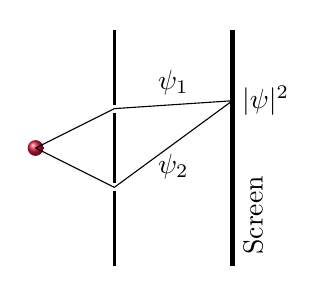
\begin{tikzpicture}
          \draw [very thick] (0,1.5) -- (0,.55) (0,.45) -- (0,-.45)
                             (0,-.55) -- (0,-1.5);
          \shade [ball color = Crimson] (-1,0) circle (.1);
          \draw (-1,0) -- (0,.5) -- (1.5,.6)
           node [midway, above] {$\psi_1$}
           (-1,0) -- (0,-.5) -- (1.5,.6) node [right] {$|\psi|^2$}
           node [midway, below] {$\psi_2$};
          \draw [ultra thick] (1.5,1.5) -- (1.5,-1.5)
           node [above right] {\rotatebox{90}{Screen}};
      \end{tikzpicture}
      \end{center}
      \end{paracol}
      The last term represents the interference between the two paths
      and is responsible for the pattern.
    \end{enumext}
    \item Stern-Gerlach experiment.
    \paragraph{Experiment Description}
    \begin{paracol}{2}
      Silver atoms are heated in an oven, then some of them
      escape from a small hole in the oven. The silver atom beam goes through
      a collimator and is then subjected to an inhomogeneous magnetic field.
      \switchcolumn
      \begin{center}
      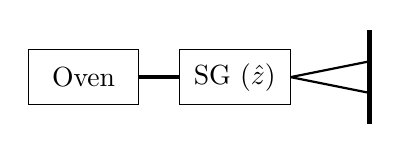
\begin{tikzpicture}
        \node [draw, minimum width = 4em, minimum height = 2em]
          (oven) at (0,0) {Oven};
        \node [draw, minimum width = 4em, minimum height = 2em, right = .5cm]
          (SG) at (oven.east) {SG ($\hat{\bm z}$)};
        \draw [very thick] (oven.east) -- (SG.west);
        \draw [thick] (SG.east) --++ (1,.2);
        \draw [thick] (SG.east) --++ (1,-.2);
        \draw [ultra thick] ([xshift = 1cm, yshift = .6cm]SG.east) --++
          (0,-1.2);
      \end{tikzpicture}
      \end{center}
    \end{paracol}
    Since the atoms in the oven are randomly oriented, people expect a continuous bundle of beams to come out of the magnetic field in the Stern-Gerlach apparatus.
    However, what the experiment observed is that the SG apparatus \emph{splits the original silver beam} from the oven \emph{into two distinct components}.
    \paragraph{Interpretation}
    The discrete deflection reveals that the electron spin is quantized.
    The magnetic moment of electrons (and thus atoms)
    can only take discrete values relative to any measurement axis.
    For electrons, the measurement of the spin component
    along any axis yields only one of two possible values:
    $+\hbar/2$ (spin up) or $-\hbar/2$ (spin down).
    \item Aharonov-Bohm effect.
    \paragraph{Experiment Description}
    \begin{paracol}{2}
      A beam of electrons is split into two paths
      (e.g., using a double-slit setup) that encircle a region
      containing a long solenoid that produces a confined magnetic field.
      The magnetic field $\bm B$ is zero outside the solenoid,
      but the magnetic vector potential $\bm A$ is non-zero outside.
      The two beams are recombined to produce interference fringes on a screen.
      \switchcolumn
      \begin{center}
        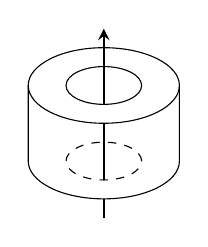
\begin{tikzpicture}[scale = .6]
          \draw (0,0) ellipse (1.6 and .8) ellipse (.8 and .4);
          \draw (-1.6,0) --++ (0,-1.6) arc (-180:0:1.6 and .8) --++ (0,1.6);
          \draw [dashed] (0,-1.6) ellipse (.8 and .4);
          \draw [thick] (0,-2.8) --++ (0,.4);
          \draw [thick] (0,-2) --++ (0,1.2);
          \draw [thick, -stealth] (0,-.4) --++ (0,1.6);
        \end{tikzpicture}
      \end{center}
    \end{paracol}

    When a current is passed through the solenoid,
    creating a magnetic flux $\Phi$ inside it,
    the interference pattern shifts \emph{even though
    the electrons travel in regions where the magnetic field is zero}.
    \paragraph{Interpretation}
    The effect highlights the non-local nature of quantum mechanics:
    electrons are influenced by the vector potential
    without entering the magnetic field region.
    The measured phase shift is gauge-invariant,
    depending on the enclosed magnetic flux,
    not the non-measurable potential itself.
  \end{enumext}
\end{solution}

% \clearpage

\begin{problem}[Optional, 30']
  Solve the hydrogen atom model:
  \[
    \mathcal H = \frac{\hat p^2}{2m} - \frac{e^2}{4 \pi \varepsilon_0} \frac1r.
  \]
\end{problem}
\begin{solution}
  Assume the wave function of hydrogen atom is
  $\Psi(r,t) = \psi(r) \upe^{-\iu\omega t}$.
  Substitute the time-independent wave function to Schr\"odinger equation
  \[
    \ab(-\frac{\hbar^2}{2m} \nabla^2 - \frac{e^2}{4\pi\varepsilon_0} \frac1r)
    \psi(r,\theta,\phi) = E \psi(r,\theta,\phi).
  \]
  Since the given hydrogen atom's potential is central,
  that is depends only on $r$, the Laplacian operator becomes
  \[
    \nabla^2 = \frac1{r^2} \pdv*{r^2 \pdv*{}r}r
             + \frac1{r^2\sin\theta} \pdv*{\sin\theta \pdv*{}\theta}\theta
             + \frac1{r^2\sin^2\theta} \pdv*[2]{}\phi.
  \]
  Referring to \emph{Mathematical Methods in Physics}, we have
  \[
    \ab(\frac1{\sin\theta} \pdv*{}\theta \sin\theta \pdv*{}\theta
  + \frac1{\sin^2\theta} \pdv*[2]{}\phi) Y_{lm}(\theta,\phi)
  = -l(l + 1) Y_{lm}(\theta,\phi).
  \]
  then we can separate the variables again. Let
  \[
    \psi(r,\theta,\phi) = R_{nl}(r) Y_{lm}(\theta,\phi),
  \]
  where $R_l(r)$ is the \emph{Radial Wave Function},
  and $Y_{lm}(\theta,\phi)$ is the spherical function. 
  Substitute $\psi(r,\theta,\phi)$ to Schr\"odinger equation, we have
  \[
    -\frac{\hbar^2}{2m} \frac1{r^2} \odv*{\ab(r^2 \odv{R_{nl}(r)}r)}r
    + \frac{\hbar^2 l (l + 1)}{2mr^2}R_{nl}(r)
    - \frac{e^2}{4\pi\varepsilon_0r} R_{nl}(r).
  \]
  Let $R_{nl}(r) = \chi_l(r)/r$, then substitute it to the Schr\"odinger equation,
  \[
    \chi''(r) + \ab[\frac{2m}{\hbar^2}\ab(E + \frac{e^2}{4\pi\varepsilon_0r})
    - \frac{l(l + 1)}{r^2}] \chi_l(r) = 0.
  \]
  To solve it, consider its asymptotic behavior first.
  \begin{enumext}[label = \roman*]
    \item When $r \to 0$, we have
    \[
      \chi_l''(r) - \frac{l(l+1)}{r^2} \chi_l(r) = 0.
    \]
    and we take the solution $\chi_l^0(r) = r^{l+1}$
    ($\chi_l^0(r) = r^{-l}$ is discard to avoid divergent).
    \item When $r \to \infty$, we have
    \[
      \chi_l''(r) + \frac{2m}{\hbar^2} E\chi_l(r) = 0
    \]
    and we take the solution $\chi_l^\infty(r) = \upe^{-kr}$,
    where $k = \sqrt{2mE/\hbar^2}$
    ($\chi_l^\infty(r) = \upe^{kr}$ is also discard).
  \end{enumext}
  To obtain the general solution, let
  \[
    \chi_l(r) = \chi_l^0(r) \chi_l^\infty(r) u_l(r).
  \]
  and substitute it to the Schr\"odinger equation
  \[
    \xi^2 \odv[2]{u_l(\xi)}\xi + [2(l + 1) - \xi] \odv{u_l(\xi)}\xi
  - \frac{2(L + 1)k - \frac{2me^2}{4\pi\varepsilon_0\hbar^2}}{2k} u_l(\xi) = 0,
  \]
  which suits the Laguerre polynomial
  \[
    \xi \odv[2]{u_l(\xi)}\xi + (\gamma - \xi) \odv{u_l(\xi)}\xi
  - \alpha u_l(\xi) = 0,
  \]
  compare with it, we have
  \[
    \gamma = 2(l + 1), \qq{and}
    \alpha = l + 1 - \frac{me^2}{4\pi\varepsilon_0 k\hbar^2}.
  \]
  Since the solution of this equation at $\xi = 0$ can be expanded into
  a series
  \[
    F_{\gamma,\alpha}(\xi)
  = 1 + \sum_{n = 1}^\infty\ab\{
    \ab[\frac{(\alpha + n - 1)!}{(\alpha - 1)!}\xi^n]\bigg/
    \ab[\frac{(\gamma + n - 1)!}{(\gamma - 1)!}n]\}.
  \]
  Apply \emph{d'Alembert's Judgement} to the $n$th
  and the $n + 1$th terms of $F_{\gamma,\alpha}(\xi)$
  \[
    \lim_{n\to\infty} \frac{f_{n+1}(\xi)}{f_n(\xi)} = \frac\xi n,
  \]
  means that $F_{\gamma,\alpha}(\xi)$ will divergent.
  To avoid this,
  the series needs to be cut off at the $n'$th term ($n'$ is finite), let
  $n' = -\alpha$, that is
  \[
    l + 1 - \frac{me^2}{4\pi\varepsilon_0 k\hbar^2} = n', \quad
    n \equiv l + 1 + n' = \frac{me^2}{4\pi\varepsilon_0 k\hbar^2},
  \]
  since $k = \sqrt{2mE/\hbar^2}$, we obtain the energy of hydrogen atom
  \[
    E_n = - \frac{me^4}{32\pi\varepsilon_0\hbar^2} \frac1{n^2}
  = -\frac{E_0}{n^2},
  \]
  and the basic state wave function is
  \[
    \psi_{100}(r,\theta,\phi) = \frac1{\sqrt{\pi a_0^3}} \upe^{-r/a_0}.
  \]
  where $a_0 = 4\pi\varepsilon_0\hbar^2/me^2$ is Bohr radius.
\end{solution}

\newweek
% !TeX root = ../main.tex

\section{Hilbert Space}

\begin{problem}[Function space]
  A square-integrable function, or $L^2$ function, is a real- or complex-valued
  function for which the integral of the square of the absolute value is finite.
  Let us consider the set of complex-valued, continuous $L^2$ functions on the real line $\mathbb R$ (or on a subset $A \subset \mathbb R$).
  The set $L^2(A) = \{\psi: A \to \mathbb C | \int_A |\psi(x)|^2 \d x < \infty\}$
  is naturally a complex vector space, called \emph{function space}.
  \begin{enumext}
    \item Show that the integral $\int_A \varphi(x)^* \psi(x) \d x$
    with $\varphi$, $\psi \in L^2(A)$ defines an \emph{inner product}
    $\braket<\varphi|\psi>$.
    \item $L^2(A)$ is a Hilbert space with the above definition of inner product.
    Find at least two different orthonormal bases (excluding $\delta$-functions)
    for each of the three cases
    \begin{enumext}[columns = 3]
      \item $A = (-\infty, +\infty)$;
      \item $A = [-1, 1]$;
      \item $A = (0, +\infty)$.
    \end{enumext}
    Demonstrate the orthonormality and the completeness explicitly.
    (Hint: One choice can be our familiar Fourier basis
    and the other from a polynomial expansion by virtue of
    \emph{Weierstrass's theorem}). Also see Problem 1.2.
  \end{enumext}
\end{problem}
\begin{solution}\leavevmode
  \begin{enumext}
    \item \begin{proof}
    To show that the integral defines an inner product, we check the axioms of an inner product on a complex vector space.
    \begin{enumext}
      \item Conjugate symmetry: $\braket<\varphi|\psi> = \int_A \varphi^*\psi
      = \overline{\int_A \psi^*\varphi} = \overline{\braket<\psi|\varphi>}$.
      \item Linearity: For $\alpha$, $\beta \in \mathbb C$,
      in the second argument,
      \[
        \braket<\varphi|(\alpha\psi_1 + \beta\psi_2)>
      = \int_A \varphi^*(\alpha\psi_1 + \beta\psi_2)
      = \alpha\braket<\varphi|\psi_1> + \beta\braket<\varphi|\psi_2>.
      \]
      Conjugate-linearity in the first argument follows similarly.
      \item Positive-definiteness: $\braket<\psi|\psi> = \int_A |\psi(x)|^2 \d x\geq 0$, also for $\varphi$.
    \end{enumext}
    Hence, $\braket<\varphi|\psi>$ is an inner product on $L^2(A)$.
    \end{proof}
    \item \begin{enumext}
      \item $A = (-\infty, +\infty)$
      \begin{enumext}[wrap-label = \underline{Case #1}, label = \arabic*,
                      list-indent = 0pt]
        \item Hermite functions
        \[
          \psi_n(x) = \frac1{\sqrt{\sqrt\pi2^nn!}} H_n(x) \upe^{-x^2/2}, \quad
          n = 0,1,2,\ldots,
        \]
        where $H_n$ is the $n-$th Hermite polynomial, belong to $L^2(\mathbb R)$.
        Using the orthonormality of the Hermite polynomial,
        we get the orthonormality of the function
        \[
          \int_A \psi_m(x) \psi_n(x) \d x = \delta_{mn}.
        \]
        From Sturm-Liouville theory,
        $\{\psi_n\}_{n\geq0}$ form a basis for $L^2(\mathbb R)$.
        So it is complete.
        \item Haar basis
        \[
          \psi_{n,k}(x) = 2^{n/2} \psi_{0,0}(2^nx - k), \quad x \in \mathbb R,
        \]
        $\psi$ is a compactly supported mother wavelet chosen so that the  family is orthonormal in $L^2(\mathbb R)$
        \[
          \int_A \psi_{n,k}(x) \psi_{n',k'}(x) \d x = \delta_{nn'}\delta{jj'}.
        \]
        The Haar system on the real line is an orthonormal basis in $L^2(\mathbb R)$, so it is complete.
      \end{enumext}
      \item $A = [-1, 1]$
      \begin{enumext}[wrap-label = \underline{Case #1}, label = \arabic*,
                    list-indent = 0pt]
        \item Fourier basis
        \[
          \psi_n(x) = \frac1{\sqrt2} \upe^{\iu n\pi x}, \quad n \in \mathbb Z,
        \]
        its orthonormality
        \[
          \int_{-1}^1 \psi_m(x) \psi_n(x) \d x
        = \frac12 \int_{-1}^1 \upe^{\iu(m-n)\pi x} \d x = \delta_{mn},
        \]
        It is standard Fourier series theory, which satisfies completeness.
        \item Legendre polynomials
        \[
          \psi_n(x) = \sqrt{n + \frac12} P_n(x), \quad n = 0, 1, 2, \ldots,
        \]
        its orthonormality
        \[
          \int_{-1}^1 \psi_m(x) \psi_n(x) \d x
        = \frac{2n + 1}{2} \int_{-1}^1 P_m(x) P_n(x) \d x = \delta_{mn}.
        \]
        Due to Weierstrass' theorem, polynomials are dense in $A$ in the sup norm, hence complete in $L^2$.
      \end{enumext}
      \item $A = (0, +\infty)$
      \begin{enumext}[wrap-label = \underline{Case #1}, label = \arabic*,
                      list-indent = 0pt]
        \item Laguerre functions
        \[
          \psi_n(x) = \upe^{-x/2} L_n(x), \qq{where}
          L_n(x) = \upe^x \odv*[n]{(x^n \upe^{-x})}x,
        \]
        its orthonormality
        \[
          \int_A \psi_m(x) \psi_n(x) \d x = \int_A \upe^{-x} L_m(x) \d x
        = \delta_{mn}.
        \]
        The Laguerre polynomials (with the $\upe^{x/2}$ factor) are eigenfunctions of a self-adjoint Sturm-Liouville operator on
        $(0, \infty)$ and form a complete orthonormal set in $L^2(0, \infty)$.
        \item Consider the mapping
        $\varphi: A \to (0,1)$, $t \mapsto \frac2\pi\arctan(t)$.
        Then use the sine functions in $x$-space
        \[
          \psi(x) = \sqrt2\sin(n\pi t(x)),
        \]
        it is trivial that sine functions are orthonormal and complete.
      \end{enumext}
    \end{enumext}
  \end{enumext}
\end{solution}

\newpage

\begin{problem}[Sturm-Liouville theory]
  Many physics problems involve second-order, linear differential equations
  of the general form: $\alpha(x) y'' + \beta(x) y' + \gamma(x) y = \lambda y$,
  where $\alpha$, $\beta$, and $\gamma$ are real functions, and $\lambda$ is a constant.
  Such an ODE can be rewritten in a \emph{Sturm-Liouville} form $\mathcal Ly = \lambda y$
  with a proper choice (cf. (a)) of the \emph{weight function} $\omega(x)$ in the linear second-order differential operator
  \[
    \mathcal L = \omega^{-1} \odv*{\ab(\omega \alpha \odv*{}x)}x + \gamma.
  \]
  This, combined with suitable boundary conditions (cf. (b)), renders $\mathcal L$
  a self-adjoint operator if the inner product is defined to be
  \[
    \braket<u|v> = \int_{x_1}^{x_2} u^*(x) v(x) \omega(x) \d x.
  \]
  Hence, the Sturm-Liouville problem becomes an eigenvalue problem with the solutions being the eigenvalues and the corresponding $\lambda$'s being the eigenvalues.
  The Sturm-Liouville theory provides a connection between a second-order, linear differential equation and Hilbert space $\mathcal L^2 ([x_1, x_2])$
  by establishing the normalized eigenvectors of the former (in its Sturm-Liouville form) as a complete orthonormal basis of the latter.
  \begin{enumext}
    \item Find the general expression of $\omega(x)$ that permits the rewriting of the original ODE in its Sturm-Liouville form.
    Compute $\omega(x)$ for the following ODEs
    \begin{alignat*}{4}
      & \qq{(i)}   && -y'' + 2xy' = \lambda y         && \qq{(Hermite)}\\
      & \qq{(ii)}  && -(1 - x^2)y''+ 2xy' = \lambda y && \qq{(Legendre)}\\
      & \qq{(iii)} && -xy'' - (1 - x)y' = \lambda y   && \qq{(Laguerre)}
    \end{alignat*}
    \item Find the general boundary condition $\mathcal L$
    to be self-adjoint in $[x_1, x_2]$ with respect to the above-defined inner product,
    namely, $\braket<u|\mathcal Lv> = \braket<\mathcal Lu|v>$.
    Note that $u$ and $v$ can, in general, be complex functions.
    Check that the boundary condition is satisfied when
    \begin{enumext}
      \item $x_1 = -\infty$, $x_2 = +\infty$ for Hermite equation.
      \item $x_1 = -1$, $x_2 = 1$ for Legendre equation.
      \item $x_1 = 0$, $x_2 = +\infty$ for Laguerre equation.
    \end{enumext}
    \item With $\mathcal L$ being self-adjoint in $[x_1, x_2]$, show that if
    $\mathcal Lv_i = \lambda_i v_i$ ($i = 1$, $2$) and $\lambda_1 \neq \lambda_2$,
    then $\braket<v_1|v_2> = 0$.
  \end{enumext}
\end{problem}
\begin{solution}\leavevmode
  \begin{enumext}
    \item Apply $\mathcal L$ to a test function $y$, we have
    \[
      \mathcal Ly = \frac1\omega[(\omega\alpha)'y' + \omega\alpha y''] + \gamma y
    = \alpha y'' + \frac{(\omega\alpha)'}{\omega}y' + \gamma y,
    \]
    Comparing with the original $\alpha y'' + \beta y' + \gamma y$, we require
    \[
      \beta(x) = \frac{(\omega\alpha)'}{\omega} = \alpha'(x) + \alpha(x) \frac{\omega'(x)}{\omega(x)}.
    \]
    Then, we can solve $\omega'/\omega$
    \[
      \frac{\omega'}{\omega} = \frac{\beta(x) - \alpha'(x)}{\alpha(x)},
      \quad
      \omega(x) = C \exp\ab(\int_A \frac{\beta(x') - \alpha'(x')}{\alpha(x')} \d x'),
    \]
    where $C$ is an arbitrary positive constant,
    and $A$ is the integral range for the following different types.
    \begin{enumext}[wrap-label* = \underline{\emph{#1}}, list-indent = 0pt]
      \item [Hermite: $-y'' + 2xy' = \lambda y$]\leavevmode\\
      To compare with, we have $\alpha = -1$, $\beta = 2x$, $\alpha' = 0$. Then
      \[
        \omega'/\omega = (2x - 0)/(-1) = -2x, \quad
        \omega(x) = C \upe^{-x^2}.
      \]
      \item [Legendre: $-(1 - x^2)y'' + 2xy' = \lambda y$]\leavevmode\\
      To compare with, we have $\alpha = -(1 - x^2)$, $\beta = 2x$, $\alpha' = 2x$.
      Then
      \[
        \omega'/\omega = (2x - 2x)/(-1), \quad \omega(x) = C.
      \]
      \item [Laguerre: $-xy'' - (1 - x)y' = \lambda y$]\leavevmode\\
      To compare with, we have
      $\alpha = -x$, $\beta = -(1 - x) = x - 1$, $\alpha' = -1$. Then
      \[
        \omega'/\omega
      = [(x - 1) - (-1)]/(-x) = -1, \quad \omega(x) = C \upe^{-x}.
      \]
    \end{enumext}
    \item Using the inner product
    \[
      \braket<u|v> = \int_{x_1}^{x_2} u^*(x) v(x) \omega(x) \d x.
    \]
    to compute the difference $\braket<u|\mathcal Lv> - \braket<\mathcal Lu|v>$.
    We have
    \begin{align*}
      \braket<u|\mathcal Lv> & = \int_{x_1}^{x_2}
      u^* \ab[\omega^{-1} (\omega \alpha v')' + \gamma v] \omega \d x
    = \int_{x_1}^{x_2} u^* (\omega \alpha v')' \d x
    + \int_{x_1}^{x_2} u^* v \gamma \omega \d x,\\
      \braket<\mathcal Lu|v> & = \int_{x_1}^{x_2}
      \ab[\omega^{-1} (\omega \alpha (u^*)' )' + \gamma u^*] v \omega \d x
    = \int_{x_1}^{x_2} (\omega \alpha (u^*)')' v \d x
    + \int_{x_1}^{x_2} \gamma u^* v \omega \d x.
    \end{align*}
    Then the difference can be expressed as
    \[
      \braket<u|\mathcal Lv> - \braket<\mathcal Lu|v>
    = \ab[\omega(x) \alpha(x) (u^*(x) v'(x) - u'^*(x) v(x))]_{x_1}^{x_2}.
    \]
    If it is zero, then $\mathcal L$ is adjoint under the corresponding interval.
    Now, substitute the three boundary conditions into the difference.
    \begin{enumext}
      \item Hermite: $x \in (-\infty, +\infty)$, $\omega = e^{-x^2}$, $\alpha = -1$.
      Boundary term: $[-e^{-x^2} (u^* v' - u'^* v)]_{-\infty}^{+\infty} = 0$.
      \item Legendre: $x \in [-1, 1]$, $\omega = 1$, $\alpha = -(1 - x^2)$.
      Boundary term $\ab[-(1 - x^2) (u^* v' - u'^* v)]_{-1}^1 = 0$.
      \item Laguerre: $x \in [0, \infty)$, $\omega = e^{-x}$, $\alpha = -x$.
      Boundary term $\ab[-x e^{-x} (u^* v' - u'^* v)]_0^{\infty} = 0$.
    \end{enumext}
    So, $\mathcal L$ is self-adjoint in the three domain.
    \item \begin{proof}
    Using self-adjointness for $i = 1$ and $i = 2$
    \[
      \lambda_2 \braket<v_1|v_2> = \braket<v_1|\mathcal L v_2>
    = \braket<\mathcal L v_1|v_2> = \lambda_1 \braket<v_1|v_2>.
    \]
    Rearranging, we can obtain
    \[
      (\lambda_2 - \lambda_1) \braket<v_1 | v_2> = 0.
    \]
    Since $\lambda_1 \neq \lambda_2$, then $\braket<v_1|v_2> = 0$.
    \end{proof}
  \end{enumext}
\end{solution}

\newpage

\begin{problem}[Linear map]
  Let $V$ and $W$ be vector spaces over the same field $\mathbb K$.
  A map $f: V \to W$ is called a \emph{linear map} if $f(au + bv) = af(u) + bf(v)$
  for all $a$, $b \in \mathbb K$ and $u$, $v \in V$.
  \begin{enumext*}[label = (\alph*)]
    \item Show that the set $L(V,W)$ of linear maps from $V$ to $W$ itself forms a vector space over $\mathbb K$.
    \item Consider finite dimensional vector spaces $V$ and $W$.
    Let $\{v_1, v_2, \ldots, v_n\}$ be a basis of $V$, and
    $\{w_1, w_2, \ldots, w_n\}$ be a basis of $W$.
    Does the set of equations $f(v_i) = \sum_{j=1}^m \omega_j F_{ji}$
    with $i = 1, 2, \ldots, n$ and $F_{ij} \in \mathbb K$ uniquely determine
    the $m \times n$ matrix $F$? Why? Conversely, does any $m \times n$ matrix $F$
    over $\mathbb K$ uniquely determine a linear map $f$ by the same set of equations? Why?
    \item Following (a) and (b), find a basis of $L(V, W)$.
    \item* (optional) Define the \emph{kernel} of $f$ to be
    $\ker(f) = \{v \in V | f(v) = 0\}$ and the \emph{image} of $f$ to be
    $\im(f) = \{\omega \in W | \omega = f(v), v \in V\}$.
    Both the kernel and the image of $f$ are vector spaces with their dimensions
    called $\text{\emph{nullity}} = \dim(\ker(f))$ and $\rank = \dim(\im(f))$, respectively.
    Prove that
    \[
      \dim(\ker(f)) + \dim(\im(f)) = \dim(V).
    \]
  \end{enumext*}
\end{problem}
\begin{solution}\leavevmode
  \begin{enumext}
    \item \begin{proof}
    Define addition and scalar multiplication on $L(V,W)$ by
    \[
      (f + g)(v) = f(v) + g(v), \quad (\alpha f)(v) = \alpha (f(v)),
    \]
    for all $f,g \in L(V,W)$, $\alpha \in \mathbb{K}$, $v \in V$.
    \paragraph{Closure and linearity}
    If $f, g$ are linear, then for all $a,b \in \mathbb{K}$ and $u,v \in V$,
      \[
      (f+g)(a u + b v) = f(a u + b v) + g(a u + b v)
    = a (f + g)(u) + b (f + g)(v),
      \]
      so $f + g$ is linear. Similarly,
      \[
        (\alpha f)(a u + b v) = \alpha (f(a u + b v)) = \alpha (a f(u) + b f(v))
      = a (\alpha f)(u) + b (\alpha f)(v),
      \]
      so $\alpha f$ is linear.
    \paragraph{Vector space axioms}
    Associativity, commutativity of addition, existence of the zero map $0: V \to W$ with $0(v) = 0_W$, additive inverses $(-f)(v) = -f(v)$, and scalar multiplication axioms all follow from the corresponding properties in $W$.
    Thus $L(V, W)$ is a vector space over $\mathbb{K}$.
    \end{proof}
    \item Let $\dim V = n$ with basis $\{v_1, \dots, v_n\}$, and $\dim W = m$ with basis $\{w_1, \dots, w_m\}$, then
    \[
    f(v_i) = \sum_{j=1}^m F_{ji}  w_j, \quad i = 1, \dots, n.,
    \]
    which defines an $m \times n$ matrix $F = (F_{ji})$.
    \begin{enumext}
      \item For fixed $i$, the coefficients $F_{1i}, \dots, F_{mi}$ are the unique coordinates of $f(v_i)$ in the basis $\{w_j\}$. So $f(v_i) = \sum_j F_{ji} w_j$ uniquely determine $F$.
      \item Define $f$ on basis vectors by $f(v_i) = \sum_{j=1}^m F_{ji} w_j$, and extend linearly: for $v = \sum_{i=1}^n a_i v_i$, define
      \[
      f(v) = \sum_{i=1}^n a_i f(v_i) = \sum_{i=1}^n \sum_{j=1}^m a_i F_{ji} w_j.
      \]
      This is well-defined and linear, and uniquely determined by $F$.
      So, any $m \times n$ matrix $F$ uniquely determine a linear map $f$,
      and there is a bijection between $L(V,W)$ and $m \times n$ matrices over $\mathbb{K}$ once bases are fixed.
    \end{enumext}
    \item Under the identification $L(V,W) \cong \mathbb{K}^{m \times n}$, define for each $1 \le p \le m$, $1 \le q \le n$ the linear map $E^{(p,q)} : V \to W$ by
    \[
      E^{(p,q)}(v_q) = w_p, \quad E^{(p,q)}(v_k) = 0 \qq{for} k \ne q,
    \]
    extended linearly.
    The matrix of $E^{(p,q)}$ has a 1 in the $(p,q)$ entry and 0 elsewhere.  
    These $mn$ maps are linearly independent and span $L(V, W)$, hence form a basis.  
    Thus
    \[
      \dim L(V,W) = m n = \dim V \cdot \dim W.
    \]
    \item \begin{proof}
    Let $f : V \to W$ be linear, $\dim V = n$; and
    let $\dim(\ker f) = k$, and choose a basis $\{u_1, \dots, u_k\}$ of $\ker f$.  
    Extend to a basis $\{u_1, \dots, u_k, u_{k+1}, \dots, u_n\}$ of $V$.
    Let $S = \{f(u_{k+1}), \dots, f(u_n)\} \subset \im f$.
    \paragraph{Span}
    For any $v \in V$, write $v = \sum_{i=1}^n a_i u_i$. Then
    \[
      f(v) = \sum_{i=1}^n a_i f(u_i) = \sum_{i=k+1}^n a_i f(u_i),
    \]
    since $f(u_1) = \dots = f(u_k) = 0$. So $\im f \subseteq \operatorname{span}(S)$.
    \paragraph{Linear independence}
    Suppose $\sum_{i=k+1}^n b_i f(u_i) = 0$. Then
    \[
      f\ab(\sum_{i=k+1}^n b_i u_i) = 0,
    \]
    so $\sum_{i=k+1}^n b_i u_i \in \ker f$.  
    Since $\{u_1, \dots, u_k\}$ is a basis of $\ker f$
    \[
      \sum_{i=k+1}^n b_i u_i = \sum_{i=1}^k c_i u_i,
    \]
    for some $c_i$. By linear independence of the full basis, all $b_i = 0$.  
    So $S$ is linearly independent.
    Thus $S$ is a basis of $\im f$, and $|S| = n - k$.  
    Hence
    \[
      \dim(\ker f) + \dim(\im f) = k + (n - k) = n = \dim V.
    \]
    which is the rank-nullity theorem.
    \end{proof}
  \end{enumext}
\end{solution}

\newpage

\begin{problem}[Coherent states]
  A coherent state $\ket|\alpha>$ is defined as an eigenstate of the annihilation
  operator $\hat a$ with a complex eigenvalue $\alpha$:
  \[
    \hat a \ket|\alpha> = \alpha \ket|\alpha>.
  \]
  \begin{enumext}
    \item Show that $\ket|\alpha> = \mathcal N\upe^{\alpha \hat a^\dagger} \ket|0>$,
    where $\mathcal N$ is a normalization constant and $\ket|0>$ is the ground state such that $\hat a\ket|0> = 0$ (review the solution of a quantum harmonic oscillator if needed).
    Compute $\mathcal N$ and $\braket<\alpha|\hat a^\dagger \hat a|\alpha>$.
    Further show that $\ket|\alpha> = \upe^{\alpha\hat a^\dagger-\alpha^*\hat a} \ket|0>$
    up to a phase factor.
    $D(\alpha) \equiv \upe^{\alpha\hat a^\dagger-\alpha^*\hat a}$
    is a unitary operator called the displacement operator because it displaces the ground state $\ket|0>$ to $\ket|\alpha>$ (note that $\ket|0>$ is a special coherent state with $\alpha = 0$).
    \item Show that the set $\{\ket|\alpha> | \alpha \in \mathbb C\}$
    form an overcomplete basis of the Hilbert space by computing
    $\braket<\alpha|\beta>$ for generic $\alpha$ and $\beta$, and proving
    \[
      \int \frac{\d^2\alpha}{\pi} \ketbra|\alpha><\alpha| = \mathbbm 1,
    \]
    where $\d^2\alpha = \d \Re\alpha \d\Im\alpha = r_\alpha \d r_\alpha\d \varphi_\alpha$ ($\alpha = \Re\alpha + \iu\Im\alpha = r_\alpha\upe^{\iu\varphi_\alpha}$).
    (Hint: Consider the matrix elements of the above operator in the orthonormal basis $\{\ket|n>\}$.)
    \item In the context of a quantum harmonic oscillator,
    $\hat a = (l^{-1}_0 \hat x + \iu l_0\hat k)/\sqrt2$,
    where $l_0 \equiv \sqrt{\hbar/m\omega}$.
    Find the wavefunction (in real space) of a coherent state $\braket<x|\alpha>$,
    and compare this wavefunction with the Gaussian wave packet we have learned in our class.
    (Hint: Consider the real-space representation of the defining equation $\hat a\ket|\alpha> = \alpha\ket|\alpha>$.)
    \item Compute $\hat U^{-1}(t,0) \hat a \hat U(t,0)$ with
    $\hat U(t,0) = \exp[-\iu(\hat a^\dagger\hat a + 1/2)\omega t]$,
    and use the result to derive $\hat U(t,0) \ket|\alpha>$.
    Interpret the result in the context of a quantum harmonic oscillator.
    (Hint: What is the physical meaning of $\Re\alpha$ and $\Im\alpha$?)
  \end{enumext}
\end{problem}
\begin{solution}\leavevmode
  \begin{enumext}
    \item \begin{proof}
    Expand the coherent state $\ket|\alpha>$ in terms of number state $\ket|n>$
    \[
      \ket|\alpha> = \sum_{n=0}^\infty c_n \ket|n>.
    \]
    Here, we merge the normalization factor into $c_n$ to simplify, and it will be released at the end. Act $\hat a$ on the expand expression of $\ket|\alpha>$, due to the property of annihilation operator
    \[
      \hat a \ket|\alpha> = \sum_{n=0}^\infty c_n \hat a \ket|n>
    = \sum_{n=1}^\infty c_n \sqrt n \ket|n - 1>
    = \alpha \sum_{n=0}^\infty c_n \ket|n>,
    \]
    the third term summing from $n = 1$ is due to $\hat a\ket|0> = 0$,
    which $n = 0$ make no sence. To uniform the lower limit of $n$,
    shift the summation index
    \[
      \hat a \ket|\alpha>
    = \sum_{n=0}^\infty c_{n+1} \sqrt{n + 1} \ket|n>
    = \alpha \sum_{n=0}^\infty c_n \ket|n>,
    \]
    then we obtain the expression of the expansion coefficient
    \[
      c_{n+1} \sqrt{n + 1} = \alpha c_n, \qq{or}
      c_n = \frac\alpha{\sqrt n} c_{n-1}
    = \frac\alpha{\sqrt n} \frac\alpha{\sqrt{n - 1}} c_{n-2} = \cdots
    = \frac{\alpha^n}{\sqrt{n!}} c_0,
    \]
    thus
    \[
      \ket|\alpha> = c_0 \sum_{n=0}^\infty \frac{\alpha^n}{\sqrt{n!}} \ket|n>
    = c_0 \sum_{n=0}^\infty \frac{(\alpha \hat a^\dagger)^n}{n!} \ket|0>
    = c_0 \upe^{\alpha \hat a^\dagger} \ket|0>,
    \]
    where $\ket|n> = \frac{(\hat a^\dagger)^n}{\sqrt{n!}}\ket|0>$.
    To get the expression of $c_0$, normalize it
    \[
      1 = \braket<\alpha|\alpha> = |c_0|^2
      \braket<0|\upe^{\alpha^*\hat a} \upe^{\alpha\hat a^\dagger}|0>
    = |c_0|^2 \sum_{n=0}^\infty \frac{|\alpha|^{2n}}{n!} \braket<n|n>
    = |c_0|^2 \upe^{|\alpha|^2}.
    \]
    Hence, we prove that
    \[
      \ket|\alpha> = \upe^{-|\alpha|^2/2} \upe^{\alpha \hat a^\dagger} \ket|0>
    = \mathcal N \upe^{\alpha \hat a^\dagger} \ket|0>,
    \]
    where $\mathcal N = c_0 = \upe^{-|\alpha|^2/2}$.
    And the ``exception value'' of $\hat a^\dagger \hat a$ under the coherent state
    \[
      \braket<\alpha|\hat a^\dagger \hat a|\alpha>
    = \alpha^*\alpha\braket<\alpha|\alpha> = |\alpha|^2,
    \]
    where $\bra<\alpha|\hat a^\dagger = \alpha^* \bra<\alpha|$.
    The displacement operator can be written as
    \[
      D(\alpha) = \upe^{\alpha \hat a^\dagger - \alpha^*\hat a}
    \xlongequal[{[\alpha\hat a^\dagger, -\alpha^*\hat a] = |\alpha|^2}]{\text{BCH identity}}
      \upe^{-|\alpha|^2/2} \upe^{\alpha \hat a^\dagger} \upe^{-\alpha^* \hat a},
    \]
    when it acts on the vacuum $\ket|0>$, to calculate it, we need to expand
    the last term $\upe^{-\alpha^* \hat a}$
    \[
      \upe^{-\alpha^* \hat a} \ket|0> = \sum_{k=0}^\infty \frac{(-\alpha^*)^k}{k!} \hat a^k \ket|0> = \ket|0>.
    \]
    Due to every $\hat a$ annihilates $\ket|0>$, so only the $k = 0$ term survives. So the result of the displacement operator acting on the vacuum is
    \[
      D(\alpha) \ket|0> = \upe^{-|\alpha|^2/2} \upe^{\alpha \hat a^\dagger} \ket|0> \equiv \ket|\alpha>.
    \]
    i.e., the overall phase convention.
    \end{proof}
    \item \begin{proof}
    Firstly, we need to calculate some identities for preparation.
    \begin{itemize}
      \item Verify $D(\alpha)$ is a unitary operator.
      \begin{equation}
        D^\dagger(\alpha) = \upe^{\alpha \hat a - \alpha^*\hat a^\dagger}
      = D(-\alpha) = D^{-1}(\alpha).\tag{A}
      \label{problem:2.4:A}
      \end{equation}
      \item Calculate $\braket<0|\upe^{\gamma \hat a^\dagger}|0>$
      \begin{equation}
        \braket<0|\upe^{\gamma \hat a^\dagger}|0>
      = \sum_{k=0}^\infty \frac{\gamma^k}{k!}\braket<0|(\hat a^\dagger)^k|0>
      = \frac{\gamma^0}{0!}\braket<0|0>
      + \sum_{k=1}^\infty \frac{\gamma^k}{k!} \sqrt{k} \braket<0|k> + \cdots
      = 1.\tag{B}
        \label{problem:2.4:B}
      \end{equation}
      Since $\braket<m|n> = \delta_{m,n}$, only $k = 0$ term survives.
      \item Calculate $\braket<m|\alpha>$ and $\braket<\alpha|n>$.
      Expand $\ket|\alpha>$ in terms of number basis
      \[
        \ket|\alpha> = \upe^{-|\alpha|^2/2} \upe^{\alpha \hat a^\dagger} \ket|0>
      = \upe^{-|\alpha|^2/2} \sum_{n=0}^\infty
        \frac{a^n}{n!} (\hat a^\dagger)^n \ket|0>
      \xlongequal[\text{Property of creation O.P.}]{(\hat a^\dagger)^n = \sqrt{n!}\ket|n>}
        \upe^{-|\alpha|^2/2} \sum_{n=0}^\infty
        \frac{a^n}{\sqrt{n!}} \ket|n>. 
      \]
      Now we obtain the inner product
      \begin{equation}
        \braket<m|\alpha> = \upe^{-|\alpha|^2/2} \sum_{n=0}^\infty
        \frac{a^n}{\sqrt{n!}} \delta_{mn}
      = \upe^{-|\alpha|^2/2} \frac{a^m}{\sqrt{m!}}, \qq{similarly}
      \braket<\alpha|n> = \upe^{-|\alpha|^2/2} \frac{(a^*)^n}{\sqrt{n!}}\tag{C}.
        \label{problem:2.4:C}
      \end{equation}
    \end{itemize}
    Now, calculate $\braket<\alpha|\beta>$. Write them in terms of the displacement operator
    \[
      \braket<\alpha|\beta> = \braket<0|D^\dagger(\alpha) D(\beta)|0>
    = \braket<0|D(-\alpha) D(\beta)|0>
    \xlongequal{\text{BCH identity}}
    \upe^{\frac12(\alpha^(\beta-\alpha\beta^*))} \braket<0|D(\beta - \alpha)|0>,
    \]
    where we used Eq. \eqref{problem:2.4:A}.
    Denote $\gamma = \beta - \alpha$ for simplification,
    using Eq. \eqref{problem:2.4:B}
    \[
      \braket<0|D(\beta - \alpha)|0> = \braket<0|D(\gamma)|0>
    \xlongequal{\text{BCH identity}} \upe^{-|\gamma|^2/2} \braket<0|\upe^{\gamma \hat a^\dagger}|0> = \upe^{-|\gamma|^2/2}.
    \]
    Substitute this equation to $\braket<\alpha|\beta>$, we have
    \[
      \braket<\alpha|\beta> = \upe^{\frac12(\alpha^*\beta-\alpha\beta^*)}
      \upe^{-|\beta-\alpha|^2/2}
    = \upe^{-\frac12|\alpha|^2-\frac12|\beta|^2+\alpha^*\beta}.
    \]
    Surround $\braket<m|n>$ to the integral kernel $\ketbra|\alpha><\alpha|$.
    The integral becomes
    \[
      \textstyle I = \braket*\big<m|\ab(\int\frac{\d^2\alpha}{\pi})|\alpha>\braket*\big<\alpha|n>.
    \]
    Substitute Eq. \eqref{problem:2.4:C} to the left and right bra-ket group, respectively
    \[
      I = \int \frac{\d^2\alpha}\pi \upe^{-|\alpha|^2} \frac{\alpha^m (\alpha^*)^n}{\sqrt{m!n!}}
      \xlongequal[m = n]{\alpha = r\upe^{\iu\theta}}
      \frac2{n!} \int_0^\infty r^{2n+1} \upe^{-r^2} \d r = 1, \qq{and}
      \int \frac{\d^2\alpha}{\pi} \ketbra|\alpha><\alpha| = \mathbbm 1,
    \]
    where the matrix element equals $\delta_{mn}$, then the operator equals the identity on the number basis.
    \end{proof}
    \item Denote the position-space wavefunction $\psi_\alpha(x) = \braket<x|\alpha>$. Act $\hat a$ on it to write the eigenvalue equation
    \[
      \frac1{\sqrt2}\ab(\frac x{l_0} + l_0 \odv*{}x) \psi_\alpha(x) = \alpha \psi_\alpha(x),
    \]
    based on $\hat a\ket|\alpha> = \alpha\ket|\alpha>$. Simplify the ODE
    \[
      \psi_\alpha' - \ab(\frac{\sqrt2\alpha}{l_0} - \frac x{l_0^2})\psi_\alpha = 0,\quad
      \psi_\alpha(x) = A\exp\ab(\frac{\sqrt2\alpha}{l_0}x - \frac{x^2}{2l_0^2}).
    \]
    Consider the real-space representation, let $\alpha = \alpha_1 + \iu\alpha_2$, and normalize it.
    We can obtain
    \[
      \psi_\alpha(x) = \frac1{(\pi l_0^2)^{1/4}}\exp\ab[-\frac{(x - x_0)^2}{2l_0^2} + \iu\frac{p_0x}{\hbar}],
    \]
    where $x_0 = \sqrt2\Re\alpha l_0$, $p_0 = \sqrt2\hbar\Im\alpha/l_0$.
    To compare with the Gaussian wave packet:
    the coherent-state wavefunction is a Gaussian wave packet centered at $x_0$ with momentum $p_0$ and width $l_0$.
    \item Apply the BCH identity, we can obtain
    \[
      \hat U^{-1}(t,0) \hat a \hat U(t,0)
    = \upe^{\iu\theta\hat N} \hat a \upe^{-\iu\theta\hat N}
    = \hat a + [\iu\theta\hat N, \hat a] + \frac1{2!}[\iu\theta\hat N, [\iu\theta\hat N, \hat a]] + \cdots
    = \hat a \sum_{n=0}^\infty \frac{(-\iu\theta)^n}{n!} = \upe^{-\iu\theta} \hat a.
    \]
    where $\hat N = \hat a^\dagger \hat a$, $\theta = \omega t$, $[\hat N, \hat a] = -\hat a$.
    Concerning $\hat U\ket|\alpha>$, which I think a violent expansion is better \textsf{:-)}
    \[
      \hat U\ket|\alpha> = \upe^{-|\alpha|^2/2} \sum_{n}^\infty \frac{\alpha^n}{\sqrt{n!}} \upe^{-\iu(n+1/2)\omega t} \ket|n>
    = \upe^{-\iu\omega t/2} \upe^{-|\alpha|^2/2} \sum_n \frac{(\alpha \upe^{-\iu\omega t})^n}{\sqrt{n!}}\ket|n>
    = \upe^{-\iu\omega t/2} \ket|\alpha \upe^{-\iu\omega t}>
    \]
    where $\hat a^\dagger \hat a \ket|n> = n\ket|n>$ and use the expression of the expansion of
    $\ket|\alpha> \to \ket|\alpha \upe^{-\iu\omega t}>$.
    The interpretation of the result said that the complex index $\alpha(t) = \alpha(0)\upe^{-\iu\omega t}$
    is the phase-space coordinate, i.e.
    \[
      \braket<x(t)> = \sqrt2l_0\Re[\alpha(t)] = x_0 \cos\theta + \frac{p_0}{m\omega}\sin\theta, ~
      \braket<p(t)> = \frac{\sqrt2\hbar}{l_0}\Im[\alpha(t)] = p_0 \cos\theta - m\omega x_0\sin\theta,
    \]
    enable the coherent-state center follows the classical harmonic-oscillator trajectory $(x(t), p(t))$
    with frequency $\omega$.
  \end{enumext}
\end{solution}

\newpage

\begin{problem}[Perturbed harmonic oscillator]
  Consider the following Hamiltonian:
  \[
    \hat H = \frac{\hbar^2\hat k^2}{2m} + \frac12m\omega^2\hat x^2 + \mathcal E(t)\hat x,
  \]
  where the last term is assumed to be a perturbation.
  \begin{enumext}
    \item For time-independent $\mathcal E(t) = \mathcal E_0$,
    compute the ground state energy and wavefunction up to the second-order correction with perturbation theory.
    Solve the model exactly and compare the exact result with the perturbative result.
    \item For time-dependent $\mathcal E(t)$, compute the transition probability
    (as a function of $t$) from the unperturbed ground state $\ket|0^{(0)}>$ to an unperturbed excited state $\ket|n^{(0)}>$ up to the second order pertubation.
    Further apply the general result to the case of $\mathcal E(t) = \mathcal E_0\sin\Omega t$, interpret what you obtain.
    \item* (optional) Solve the time-dependent model exactly and compare the exact result with the perturbative result.
    (Hint: Consider $\hat a(t)$ and $\hat n(t)$ in the Heisenberg picture, also see Problem 3(d) above.)
  \end{enumext}
\end{problem}
\begin{solution}\leavevmode
  \begin{enumext}
    \item \textbf{Perturbation theory}\\
    The coordinate operator can be written in terms of annihilation and creation operators
    \[
      \hat x = \sqrt{\frac{\hbar}{2m\omega}} (\hat a + \hat a^\dagger).
    \]
    \begin{enumext}
      \item First-order energy
      \[
        E_0^{(1)} = \braket<0^{(0)}|\mathcal E_0 \hat x|0^{(0)}> = 0.
      \]
      where $\braket<0|\hat a|0> = \braket<0|\hat a^\dagger|0> = 0$.
      \item Second-order energy
      \[
        E_0^{(2)} = \sum_{k\neq 0} \frac{|\braket<k^{(0)}|\mathcal E_0\hat x|0^{(0)}>|^2}{E_0^{(0)} - E_k^{(0)}}
      \xlongequal{\text{only $k=1$ survives}} \frac{\mathcal E_0^2 \hbar}{2m\omega}
        \frac{|\braket<1^{(0)}|1^{(0)}>|^2}{\frac12\hbar\omega - \frac32\hbar\omega}
      = -\frac{\mathcal E_0^2}{2m\omega^2}.
      \]
    \end{enumext}
    So, the perturbative result of the ground state energy up to second order gives
    \[
      E_0 \approx \frac12\hbar\omega + 0 - \frac{\mathcal E_0^2}{2m\omega^2}
    = \frac12\hbar\omega - \frac{\mathcal E_0^2}{2m\omega^2}.
    \]
    The perturbative result of the ground state wavefunction up to second order gives
    \def \0#1#2{\braket<#1^{(0)}|\mathcal E_0\hat x|#2^{(0)}>}%
    \def \1#1#2{E_#1^{(0)} - E_#2^{(0)}}%
    \begin{alignat*}{2}
      \ket|0> & \approx \ket|0^{(0)}>
      \begin{aligned}[t]
        & + \underbrace{\sum_{k\neq 0} \ket|k^{(0)}> \frac{\0k0}{\10k}}_\text{$k = 1$ survives}
          + \underbrace{\sum_{k\neq 0}\sum_{l\neq 0} \ket|k^{(0)}> \frac{\0kl\0l0}{(\10k)(\10l)}}_\text{$l = 1$, $k = 2$ survive}\\
        & - \underbrace{\sum_{k\neq 0} \ket|k^{(0)}> \frac{\0k0\000}{(\10k)^2}}_\text{Vanish}
        - \underbrace{\frac12 \ket|0^{(0)}> \sum_{k\neq0} \frac{|\0k0|^2}{(\10k)^2}}_\text{$k = 1$ survives}\\
      \end{aligned}\\
    & = \ket|0> - \alpha\ket|1> - \frac{\alpha^2}{\sqrt2} \ket|2> - \frac{\alpha^2}{2} \ket|0>,
    \end{alignat*}
    where $\alpha = \frac{\mathcal E_0}{\sqrt{2m\hbar\omega^3}}$.\pagebreak
 
    \textbf{Exact solution}\\
    The Hamiltonian can be written as
    \[
      \hat H = \frac{p^2}{2m} + \frac12m\omega^2\ab(\hat x + \frac{\mathcal E_0}{m\omega^2})^2
    - \frac{\mathcal E_0^2}{2m\omega^2}.
    \]
    shows that under this perturbation term, the spectrum is that of an H.O. center at
    $x_0 = -\frac{\mathcal E_0}{m\omega^2}$, and the eigenvalue shifted a constant of $-\frac{\mathcal E_0^2}{2m\omega^2}$.
    So, the exact ground state energy and wavefunction are
    \[
      E_0^\text{exact} = \frac12\hbar\omega - \frac{\mathcal E_0^2}{2m\omega^2},
      \quad
      \psi_0^\text{exact}(x) = \phi_0\ab(x + \frac{\mathcal E_0}{m\omega^2})
    = \ab(\frac{m\omega}{\pi\hbar})^{1/4}
      \exp\ab[-\frac{m\omega}{2\hbar} \ab(x + \frac{\mathcal E_0}{m\omega^2})^2],
    \]
    where $\phi_0(x)$ is the unperturbed H.O. ground-state wavefunction (centered at $x = 0$).\\
    \textbf{Comparison}\\
    The exact and perturbative (up to second order) energies agree.
    The exact wavefunction is the H.O. ground state shifted by $-\frac{\mathcal E_0}{2\omega^2}$
    and the perturbative corrections reproduce the expansion of that displacement.
    \item The system starts in the unperturbed ground state $\ket|\psi(0)> = \ket|0^{(0)}>$.
    $\ket|\psi(t)>$ can be expanded as
    \[
      \ket|\psi(t)> = \sum_n \ket|n^{(0)}>\braket<n^{(0)}|\psi(t)>
    \xlongequal{\text{Interaction picture}}
      \sum_n c_n(t) \upe^{-\iu E_n^{(0)}t/\hbar} \ket|n^{(0)}>.
    \]
    Thus, the probability to find the system in the unperturbed eigenstate $\ket|n^{(0)}>$
    at time $t$ is The probability is the square of the projection of $\ket|n^{(0)}>$ to $\ket|\psi(t)>$
    \[
      P_{0\to n}(t) = |\braket<n^{(0)}|\psi(t)>|^2 = |c_n(t)|^2.
    \]
    where $c_n(t)$ satisfies the Dyson series
    \[
      c_n(t) = c_n^{(0)}(t) + c_n^{(1)}(t) + c_n^{(2)}(t) + \cdots,
    \]
    we need to calculate the first and second orders.
    \begin{enumext}
      \item The first order term $c_n^{(1)}(t)$\\
      Substitute the expansion of $\ket|\psi(t)>$ to the Schr\"odinger equation,
      then inner product with $\bra<m|$, we can obtain
      \[
        \iu\hbar \dot c_m(t) = \sum_n V_{mn}(t) \upe^{\iu\omega_{mn}t} c_n(t),
      \]
      where $V_{mn}(t) = \braket<m|\hat V(t)|n>$, $\omega_{mn} \equiv (E_m - E_n)/\hbar$,
      and the relation $\hat H_0\ket|n> = E_n\ket|n>$ and the orthonormality are applied.
      Since we need to keep the order of $V$ the same on LHS and RHS,
      i.e., handle the map of different orders of corrections from LHS to RHS,
      we insert the parameter $\lambda$
      \[
        c_n(t) = \sum_{k\geq0} \lambda^k c_n^{(k)}(t).
      \]
      Then substitute it into the Schr\"odinger equation, we can have
      \[
        \iu\hbar \sum_{k\geq0} \lambda^k \dot c_n^{(k)}(t)
      = \sum_{l\geq0} \lambda^{l+1} \sum_m V_{nm}(t) \upe^{\iu\omega_{nm}t} c_m^{(l)}(t).
      \]
      Since $c_n(0) = \braket<n|0> = \delta_{n0} \equiv c_n^{(0)}(t)$, for the coefficient of $\lambda^1$
      \[
        \iu\hbar \dot c_n^{(1)}(t) = \sum_m V_{nm}(t) \upe^{\iu\omega_{nm}t} c_m^{(0)}(t)
      = V_{n0}(t) \upe^{\iu\omega_{n0}t}.
      \]
      Integral over $t$, we can obtain
      \[
        c_n^{(1)}(t) = -\frac\iu\hbar \int_0^t \d t' V_{n0}(t') \upe^{\iu\omega_{n0}t'}
      \xlongequal{\hat V(t) = \mathcal E(t) \hat x}
        -\frac\iu\hbar \sqrt{\frac\hbar{2m\omega}} \int_0^{t} \d t' \mathcal E(t') \upe^{\iu\omega t'}
      \equiv c_1^{(1)}(t),
      \]
      and the first-order transition probability to $\ket|n> = \ket|1>$ is
      \[
        P_{0\to1}^{(1)}(t) = |c_n^{(1)}(t)|^2 = \frac1{2m\omega\hbar}
        \ab|\int_0^t \d t' \mathcal E(t') \upe^{\iu\omega t'}|^2,
      \]
      where due to $\braket<n|\hat x|0>$ is nonzero only for $n = 1$.
      \item The second order term $c_n^{(2)}(t)$\\
      Similarly, the general second-order amplitude is
      \[
        c_n^{(2)}(t) = -\frac1{\hbar^2} \sum_m \braket<n|\hat x|m> \braket<m|\hat x|0>
        \int_0^t \d t' \int_0^{t'} \d t'' \mathcal E(t') \mathcal E(t'')
        \upe^{\iu\omega_{nm}t'} \upe^{\iu\omega_{m0}t''}.
      \]
      Since $m = 1$, and $n$ can be valued as $0$ or $2$, then we have
      \begin{align*}
        c_2^{(2)}(t) & = \frac1{\sqrt2m\hbar\omega} \int_0^t \d t' \int_0^{t'} \d t''
        \mathcal E(t') \mathcal E(t'') \upe^{\iu\omega(t'+t'')},\\
        c_0^{(2)}(t) & = \frac1{2m\hbar\omega} \int_0^t \d t' \int_0^{t'} \d t''
        \mathcal E(t') \mathcal E(t'') \upe^{-\iu\omega(t'-t'')}.
      \end{align*}
      and the corresponding second-order transition probabilities are
      \begin{align*}
        P_{0\to2}^{(2)} = |c_2^{(2)}(t)|^2 & = \frac1{2(m\hbar\omega)^2}
        \ab|\int_0^t \d t' \int_0^{t'} \d t''
        \mathcal E(t') \mathcal E(t'') \upe^{\iu\omega(t'+t'')}|^2,\\
        P_{0\to0}^{(2)} = |c_0^{(2)}(t)|^2 & = \frac1{(2m\hbar\omega)^2}
        \ab|\int_0^t \d t' \int_0^{t'} \d t''
        \mathcal E(t') \mathcal E(t'') \upe^{-\iu\omega(t'-t'')}|^2.
      \end{align*}
    \end{enumext}
    Now apply $\mathcal E(t) = \mathcal E_0 \sin(\Omega t)$, the first-order and second-order amplitude to $\ket|1>$ are
    \begin{align*}
      c_1^{(1)}(t) & = -\frac{\mathcal E_0}{2\hbar} \sqrt{\frac\hbar{2m\omega}}
      \ab[\frac{\upe^{\iu(\omega+\Omega)t} - 1}{\omega + \Omega} -
          \frac{\upe^{\iu(\omega-\Omega)t} - 1}{\omega - \Omega}],\\
      c_2^{(2)}(t) & = \frac{\sqrt2\mathcal E_0^2}{8m\hbar\omega}
      \ab[\frac{\upe^{\iu(\omega-\Omega)t} - 1}{\omega - \Omega} -
          \frac{\upe^{\iu(\omega+\Omega)t} - 1}{\omega + \Omega}
      ]^2,\\
      c_0^{(2)}(t) & =
      \frac{\mathcal E_0^2}{8m\hbar\omega(\omega^2 - \Omega^2)}\Bigg\{
        2\omega t + \frac\iu{2\Omega}\ab[(\omega + \Omega)\upe^{-2\iu\Omega t}
      - (\omega - \Omega) \upe^{2\iu\Omega t} - 2\Omega]\\
      & \quad + 2\iu\Omega\ab(
        \frac{1 - \upe^{-\iu(\omega+\Omega)t}}{\omega + \Omega} -
        \frac{1 - \upe^{-\iu(\omega-\Omega)t}}{\omega - \Omega})
      \Bigg\}.
    \end{align*}
    \textbf{Interpretation}
    If $\Omega \approx \omega$, then we will find that $|c_1^{(1)}|$, $|c_2^{(2)}| \propto t^2$ at short times.
    In the long-time limit, this becomes the usual resonance: the transition rate arrives at the maximum value.
    Of course, we can know the trend of $c_0^{(2)}$ from the relation $|c_0^{(2)}|^2 \approx 1 - |c_1^{(1)}|^2 - |c_2^{(2)}|^2$.
    \item The Heisenberg EOM for $\hat a(t)$ is
    \[
      \odv{\hat a}t = \frac\iu\hbar [\hat H, \hat a]
    = -\iu\omega\hat a + \frac\iu\hbar[\mathcal E(t)\hat x, \hat a]
    = -\iu\omega\hat a - \iu\frac{\mathcal E(t)}{\sqrt{2m\hbar\omega}},
    \]
    where $[\hat x, \hat a] = -\sqrt{\frac\hbar{2m\omega}}$.
    So, the solution is
    \[
      \hat a(t) = \hat a(0) \upe^{-\iu\omega t}
    - \frac\iu{\sqrt{2m\hbar\omega}} \int_0^t \d t' \mathcal E(t') \upe^{-\iu\omega(t-t')}.
    \]
    In Heisenberg picture, the state is fixed at $\ket|0>$, but $\hat a(t)$ is time-dependent;
    In Schr\"odinger picture, the state evolves. For a linear driving term, the ground state evolves into a coherent state $\ket|\alpha(t)>$ satisfying
    \[
      \hat a\ket|\psi(t)> = \alpha(t) \ket|\psi(t)>,
    \]
    where $\alpha(t)$ is the expectation value $\braket<\hat a(t)>$ in the Heisenberg picture with initial state $\ket|0>$
    \[
      \alpha(t) = \braket<0|\hat a(t)|0> = -\frac\iu{\sqrt{2m\hbar\omega}} \upe^{-\iu\omega t}
      \int_0^t \mathcal E(t') \upe^{\iu\omega t'} \d t'.
    \]
    Then, the probability is expressed as
    \[
      P_{0\to n}(t) = |\braket<n|\alpha(t)>|^2
    = \ab|{\upe^{-|\alpha|^2/2}
            \sum_{k=0}^\infty \frac{a^k}{\sqrt{k!}}\braket<n|k>}|^2
    = \upe^{-|\alpha(t)|^2} \frac{|\alpha(t)|^{2n}}{n!}.
    \]
    For small $\mathcal E_0$, $\alpha(t)$ is small, so
    \[
      P_{0\to1} \approx |\alpha(t)|^2, \qq{and} P_{0\to2} \approx \frac12|\alpha(t)|^4.
    \]
    So perturbation theory to second order matches the exact expansion after expanding in terms of $\alpha(t)$.
  \end{enumext}
\end{solution}

\newpage

\begin{problem}[Quantum foundations]
  Referring to the reading material ``Addressing the quantum measurement problem''
  by Sean M. Carroll (attached below),
  which of the following types of theories is your favorite?
  (Maybe tell me why? Or do you have your own alternative theory?)
  \begin{enumerate*}
    \item epistemic;
    \item hidden-variable;
    \item objective-collapse;
    \item Everett's many-worlds.
  \end{enumerate*}
\end{problem}
\begin{solution}
  My favorite theory is \textbf{Everett's Many-Worlds theory}.

  What makes this interpretation most appealing is its simplicity and consistency. It treats the wavefunction as a complete description of reality that always evolves according to the Schr\"odinger equation—no mysterious collapses or hidden mechanisms are required. In this view, measurement is just a physical interaction that entangles a system with its environment, causing the universal wavefunction to branch into different components, each corresponding to a possible outcome.

  Of course, the idea of a constantly branching multiverse may initially sound extravagant. However, modern decoherence theory makes it more tangible by explaining why these branches become effectively independent and why we only experience one of them. I also appreciate that Many-Worlds doesn't add extra postulates—rather, it takes quantum mechanics at face value and follows its logic wherever it leads.

  Nonetheless, this interpretation isn't free of problems. The biggest challenge is the probability issue: if every outcome occurs somewhere, how do we make sense of the Born rule? And although it's admittedly strange to think there could be countless versions of ourselves living in parallel worlds, I still find Many-Worlds the most compelling. It offers a clean and coherent picture of quantum reality and addresses the measurement problem head-on, without compromise.
\end{solution}

\clearpage

\setcounter{problem}{0}
\begin{problem}[Function space]
\end{problem}
\begin{solution}[By TA]\leavevmode
  \begin{enumext}
    \item \[
      \int_A |\psi(x)|^2 \d x
    \]
    To prove the three properties: Conjugate, Linearity,
    and Positive-definiteness.
    \item Fourier bases.
    \begin{enumext}
      \item $(-\infty, +\infty)$, the wavefunction
      $\{\braket<x|k> = \frac1{\sqrt{2\pi}}\upe^{\iu kx}\}$,
      $\alpha \sim k \in \mathbb R$.
      The normalization
      \[
        \int_{-\infty}^{+\infty} \psi_k(x)^* \psi_k(x) \d x = \delta(k - k'),
      \]
      The orthonormality
      \[
        \int_{-\infty}^{+\infty} \psi_k(x) \psi_k(x') \d k = \delta(x - x')
      \]
      \begin{remark}[For $\{\ket|\alpha>\}$]
        Orthonormality
        \[
          \braket<\alpha|\alpha'> = \delta_{\alpha\alpha'} \to
          \int \d x \alpha^*(x) \alpha'(x) = \delta_{\alpha\alpha'}
        \]
        Completeness
        \[
          \sum_\alpha \ketbra|\alpha><\alpha| = \identity \to
          \sum_\alpha \braket<x|\alpha>\braket<\alpha|x'> = \delta(x - x')
        \]
      \end{remark}
      \begin{remark}[Or Haar basis:]
      \[
        \phi(x) = \begin{cases}
          1, & 0 \leq x \leq 1,\\
          0, & \text{otherwise}
        \end{cases}, \quad
        \psi(x) = 
        \begin{cases}
          1, & 0 \leq x \leq \frac12,\\
          -1, & \frac12 \leq x < 1,\\
          0, & \text{otherwise}
        \end{cases}, \quad
        \psi_{j,k}(x) = 2^{j/2} \psi(2^jx - k), \quad j, k \in \mathbb Z
      \]
      \end{remark}
      \item $[-1, 1]$
      \begin{paracol}{2}
      The wavefunction
      \[
        \upe^{\iu k x}
      \]
      Then, $k \cdot \Delta x = n \cdot 2\pi$, $k_n = n\pi$. The basis
      \[
        \ab\{\frac1{\sqrt2} \upe^{\iu n\pi x}\}, \quad \alpha \sim n
      \]
      \switchcolumn \centering
      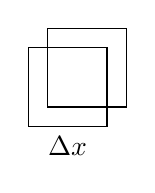
\begin{tikzpicture}
        \draw (0,0) rectangle (1,1);
        \draw (.25,.25) rectangle (1.25,1.25);
        \node [below] at (.5,0) {$\Delta x$};
      \end{tikzpicture}
      \end{paracol}
      \item $(0, +\infty)$. The basis
      \[
        \ab\{\sqrt{\frac2\pi} \cos(kx), \quad \alpha \sim k \in \mathbb R^+\}
      \]
    \end{enumext}
  \end{enumext}
\end{solution}
\begin{problem}[Strum-Liouville theory]
\end{problem}
\begin{solution}[By TA]\leavevmode
  \begin{enumext}
    \item Actually, the problem is something like
    \[
      \braket<u|v> = \int_{x_1}^{x_2} u^*(x) v(x) \omega(x) \d x, \qq{where}
      \alpha(x),\ \beta(x),\ \gamma(x) \in \mathbbm R
    \]
    The operator
    \[
      \mathcal L = \omega^{-1} \odv*[fun]{\omega\alpha \odv*{}x}x + \gamma
    = \alpha \odv*[2]{}x + \omega^{-1} \odv*[fun]{\omega\alpha}x + \gamma
    \]
    Then,
    \[
      \alpha(x)y'' + \beta(x)y' + \gamma(x)y = \lambda y, \quad
      \beta(x) = \omega^{-1} \odv*[fun]{\omega\alpha}x \Rightarrow
      \frac{\beta\omega\alpha}{\alpha} = \odv[fun]{\omega\alpha}x, \Rightarrow
      \omega = \frac C\alpha \upe^{\int\frac\beta\alpha \d x}
    \]
    Or, it can be a extension of the inner product.
    \begin{enumext}[columns = 3]
      \item $\omega(\alpha) = C\upe^{-x^2} \sim \upe^{-x^2}$
      \item $\omega(x) = C \sim 1$.
      \item $\omega(x) = C\upe^{-x} \sim \upe^{-x}$.
    \end{enumext}
    \item Calculate directly
    \[
      \braket<u|\mathcal Lv> = \braket<\mathcal Lu|v>, \quad
      \omega \in \mathbb R
    \]
    Then, we will obtain
    \[
      \mathcal \omega\alpha(u^*v' - u'^*v)\big|_{x_1}^{x_2}, \quad
      \omega(x_2)\alpha(x_2) = \omega(x_1)\alpha(x_1) = 0
    \]
    \begin{enumext}
      \item $(-\infty, +\infty)$
      \[
        H_n(x) = (-1)^n \upe^{x^2} \odv*[n]{\upe^{-x^2}}x, \quad
        \upe^{-t^2+2xt} = \sum_{n=0}^\infty \frac{k\ln(x)}{n!}t^n
      \]
      \item $[-1, 1]$
      \[
        P_n(x) = \frac1{2^nn!} \odv*{(x^2 - 1)^n}x, \quad
        \frac1{\sqrt{t^2 - 2xt + 1}} = \sum_{n=0}^\infty P_n(x)t^n
      \]
      \item 
      \[
        L_n(x) = \frac1{n!} \upe^x \odv*[n,fun]{\upe^{-x} x^n}x, \quad
        \frac1{1 - t} \upe^{-\frac{tx}{1-t}} = \sum_{n=0}^\infty \ln(x) t^n
      \]
    \end{enumext}
    \item Write the eigenfunctions
    \[
      \mathcal Lv_i = \lambda_i v_i, \quad
      \braket<\mathcal Lv_1|v_2> = \braket<v_1|\mathcal Lv_2>
    \]
    then,
    \[
      (\lambda_1 - \lambda_2)\braket<v_1|v_2> = 0, \quad
      \lambda_1 \neq \lambda_2,
      \Rightarrow \braket<v_1|v_2> = 0
    \]
  \end{enumext}
  \begin{remark}
    Actually, an arbitrary function can be exapnded as
    \[
      f(x) = c_01 + c_1 x + c_2 x^2 + \cdots + c_nx^n + \cdots
    \]
    when one write it, he assumed that
    \[
      \{1, x, x^2, x^3, \cdots, x^n, \cdots\}
    \]
    has constructed a basis of $f(x)$. But they are not orthonormal.
    We need to make the orthonormality between every two elements by
    Scimet orthonormality, for example, in range $[0,1]$
    \[
      \int_{A \sim \mathbbm R} \d x \varphi^*(x) \chi(x) = \braket<\varphi|\chi>
    \]
    If the range is $\mathbbm R$, the integral $\int_{\mathbbm R} x^{n+m}$ makes
    no sense. We need to make it square integral on the real axis by
    multiplying, it would be something like a Gaussian function
    $\omega(x) \sim \upe^{-x^2}$. Then, the integral becomes
    \[
      \int_\infty \d x \omega(x) x^{n+m} = 0
    \]
    To ``kill'' the functioin on both sides, or add the weight function
    $\omega = \upe^{-x}$ to kill the function on one side.
  \end{remark}
\end{solution}
\begin{problem}[Linear map]
\end{problem}
\begin{solution}[By TA]\leavevmode
  \begin{enumext}
    \item $L:\ V \to W$. Vector space $f(u)$
    \begin{enumext}
      \item $+$: identity, inverse, commutativity;
      associativity: $(f_1 + f_2) + f_3 = \cdots$
      \item $\times$: $a(bf_1) = (ab)f_1$ 
      \item $+\times$: $a(f_1 + f_2)$, $(a + b)f_1$
    \end{enumext}
    \item $V$ and $W$ are two matrix, the transformation between is a matrix,
    actually, a linear map. The matrix is JUST A TOOL.
    \[
      \bm v = \sum_{i=1}^{\dim(V)} c_i \bm v_i
    \]
    The core formula is
    \[
      f(v_i) = \sum_{j=1}^n w_i F_{ji} \equiv \bm u_i
    \]
    Which can be written into matrix
    \[
      (w_1, w_2, \cdots, w_n)
      \pxmat[showtop = 1, showleft = 1]Fmn =
      (u_1, u_2, \cdots, u_n)
    \]
    Uniqueness: The two vectors are unique, then, the matrix is unique.
    \item For example
    \[
      \begin{pmatrix}
        a & b\\ c& d
      \end{pmatrix} = \sum_{i=1}^4 f_i M_i
      = a\begin{pmatrix}
        1 & 0\\0 & 0
      \end{pmatrix} + b\begin{pmatrix}
        0 & 1\\0 & 0
      \end{pmatrix} + \begin{pmatrix}
        0 & 0\\1 & 0
      \end{pmatrix} + d\begin{pmatrix}
        0 & 0\\0 & 1
      \end{pmatrix}
    \]
    We can write
    \[
      A = \{F^{kl}, 1 \leq k \leq n,\ 1 \leq l \leq m\}, \quad
      F^{kl}(\bm V_i) = \bm W_j \delta_{ik} \delta_{jl}
    \]
    \item By definition
    \begin{align*}
      \ker(f) & = \{v \in V|f(v) = 0\}\\
      \im(f)  & = \{w\in W|w = f(v), v \in V\}\\
      \dim(\ker(f)) & = s, \quad \dim(\im(f)) = m, \quad \dim(V) = g
    \end{align*}
    and prove $s + m = g$.
    We can write
    \[
      S = \{v_1, v_2, \ldots, v_s\}, ~ f(v) = 0, \quad
      M = \{v_{s+1}, \ldots, v_g\},  ~ f(v) = w
    \]
    For arbitrary $v$, $f(v) = 0$, it means a linear combination
    \[
      v = \sum_{i=1}^s c_iv_i, \quad v_i \in S
    \]
    Then, $f(v) = w \in W \Rightarrow v = \sum_{i=g+1}^g c_iv_i$, $v_i \im M$.
    Substitute
    \[
      f(\bm v) = f\ab(\sum_{i=s+1}^g c_i \bm v_i)
    = \sum_{i=s+1}^g c_i f(\bm v_i)
    = \sum_{i=s+1}^g c_i \underbrace{f(\bm v_2)}_{w_i}
    \]
    Then, consider $v_{1 -- 3}$ and $w_{1 -- 3}$. Let
    \[
      w_1 = aw_2 + bw_3, \quad
      f(v_1) = af(v_2) + bf(v_3), \quad = v_1 = av_2 + bv_3
    \]
    Then, we can prove the dim of $W$-space. $s + m = g$.
    \paragraph{Interuption}
    \[
      (w_1, w_2, \cdots, w_n)
      \pxmat[showtop = 1, showleft = 1]Fmn =
      (u_1, u_2, \cdots, u_n)
    \]
    where the top three cols of $F$ is $0$.
  \end{enumext}
  \begin{remark}
    $f:\ V\to W$. The kernel.
    \[
      \ker(f) = \{v\in V|f(v) = 0_w\}
    \]
    conduct the linear space.
    The linear space always is
    \[
      (v, F) = (+, \times)
    \]
    about elements or operations.
    If $v_1$, $v_2 \in \ker(f)$ then $av_1 + bv_2 \in \ker(f)$, $a$, $b \in F$.
    i.e., $\ker$ is a linear space, also,
    the $\im(f) = \{w\in W|\exists u\in V, w = f(u)\} < w$.
    Also, we can separate an arbitrary vector in $V$
    \begin{center}
      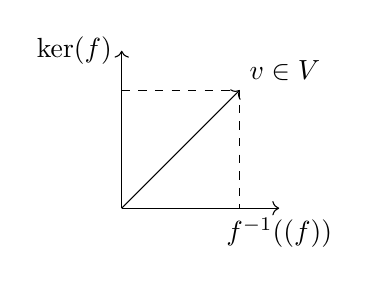
\begin{tikzpicture}
        \draw [->] (0,0) -- (2,0) node [below] {$f^{-1}(\im(f))$};
        \draw [->] (0,0) -- (0,2) node [left] {$\ker(f)$};
        \draw [->] (0,0) -- (1.5,1.5) node [above right] {$v \in V$};
        \draw [dashed] (0,1.5) -- (1.5,1.5) -- (1.5,0);
      \end{tikzpicture}
    \end{center}
  \end{remark}
\end{solution}
\begin{problem}[Coherent states]
\end{problem}
\begin{solution}[By TA]\leavevmode
  \paragraph{Baker-Campbell-Hausdorff}
  \[
    D(\alpha) \equiv \upe^{\alpha\hat a^\dagger - \alpha^*\hat a}
  = \upe^{\alpha\hat a^\dagger} \upe^{-\alpha^*\hat a}
    \upe^{-\frac12[\alpha\hat a^\dagger, \alpha^*\hat a]}
  \]
  \begin{enumext}
    \item By definition
    \[
      \hat a\ket|\alpha> = \alpha\ket|\alpha>
    \]
    Expand it
    \[
      \ket|\alpha> = \sum_{n=0}^\infty c_i \ket|n>
    \]
    Then,
    \[
      \hat a\ket|\alpha> = \sum_{n=0}^\infty c_{n+1} \sqrt{n+1} \ket|n>
    = \alpha \sum_{n=0}^\infty c_n \ket|n>
    \]
    The coefficients
    \[
      c_{n+1}\sqrt{n + 1} = \alpha c_n, \quad
      c_n = \frac{\alpha^n}{\sqrt{n!}} c_0
    \]
    Then, the coherent state can be written as the sum of fork basis
    \[
      \ket|\alpha> = N \sum_{n=0}^\infty \frac{\alpha^n}{\sqrt{n!}} \ket|n>
    \]
    where
    \[
      \ket|n> = \frac1{\sqrt{n!}} (a^\dagger)^n \ket|0>
    \]
    So,
    \[
      \ket|\alpha> = N\sum_{n=0}^\infty
      \frac{(\alpha\hat a^\dagger)^n}{n!}\ket|0>
    \]
    \item Normalization $\braket<\alpha|\alpha>_\alpha = 1$, insert the operator
    \[
      \braket<\hat a^\dagger \hat a|\alpha>
    = (\hat a\ket|\alpha>)^\dagger\hat a\ket|\alpha> = |\alpha|^2
    \]
    Then,
    \[
      \ket|\alpha> = D(\alpha) \ket|0>
    \]
    Finally,
    \[
      \upe^{-\frac12|\alpha|^2\upe^{\alpha\hat a^\dagger}
      \cancelto{\identity}{\upe^{-\alpha^*\hat a}}}\ket|0> \to \identity
    + \hat a
    \]
    \item $\{\ket|\alpha> | \alpha \in \mathbb C\}$ overcomplete.
    $\braket<\alpha|\beta> \neq 0$,
    $\int \frac{\d^2\alpha}{\pi} \ketbra|\alpha><\alpha| = \identity$.
    \[
      \braket<n|\int\frac{\d^2\alpha}{\pi}|\alpha> \braket<\alpha|m>
    = \delta_{nm}
    = \frac1\pi \frac1{\sqrt{n!m!}} \int_0^\infty \d r r^{n+m+1}
      \upe^{-r^2} \int_0^{2\pi} \d\varphi \upe^{\iu\varphi(n-m)}
    = 2\pi\delta_{nm} \xlongequal{n=m} \delta_{nm}
    \]
    \item $\psi_\alpha(x) = \braket<x|\alpha>$.
    \[
      \braket<x|\hat a|\alpha> = \alpha \psi_\alpha(x)
    = \frac1{\sqrt2} \ab(\frac x{l_0} + l_0 \pdif x) \psi_\alpha(x)
    \]
    It is an ODE. The solution is
    \[
      \psi_\alpha(x) = k\exp\ab\{
        \ab(-\frac12\frac x{l_0} - \sqrt2\Re[\alpha])^2
       + \iu\sqrt2\Im[\alpha] \frac x{l_0}\}
    \]
    where $k = (\pi l_0^2)^{-1/4}$.

    The exponitional term
    \[
      \upe^{\frac{(x - x_0)^2}{2\sigma^2} + \iu\frac{p_0}{\hbar}x}
    \]
    The first part means the center of the wavefunction is $x_0$;
    The second term: By Fourier transformation
    \[
      \tilde\psi_\alpha(p)
    = N \int_{-\infty}^\infty \psi_\alpha(x) \upe^{-\iu px/\hbar} \d x
    \propto \upe^{-\frac{(p-p_0)^2}{2\sigma_p^2} + \iu x_0 \frac p\hbar}
    \]
    Means that in the momentum space, centered with $p_0$.
    The position and momentum is closely connected with each other.

    Actually, for coherent state,
    it should be $\upe^{-\frac1{2a}(x - x_c)^2}$ where $a = \Delta x$,
    corresponding to $\Delta p$.
    If define $l_0 = \sqrt{\frac\hbar{m\omega}}$, then $x \sim l_0$,
    $k\sim l_0^{-1}$.
    
    Coherent state vs squeezed state.
    Usually, $\braket<\alpha|\beta> \neq 0$, then define
    $P(\alpha) = |\braket<\alpha|\alpha_0>|^2$.
    The wavepack's centre is (the real part of on $x$ axis,
    or the image part of $k$ axis) $\alpha_0$.
  \end{enumext}
\end{solution}
\begin{problem}[Perturbed harmonic oscillator]
\end{problem}
\begin{solution}[By Li Jian]\leavevmode
  \begin{enumext}
    \item Time-independent:
    $V = \epsilon_0 \hat x
       = \frac{\epsilon_0}{\sqrt2}(\hat a + \hat a^\dagger)$.
    We can consider it as an electric field: the oscillator have a positive
    charge, then the electric potential is gradient.

    In classical situation, just change the equilibirum point.
    In quantum situation, to the exact solution, just merge
    \[
      H = \frac12 m\omega^2 (x - x_0)^2 + C
    \]
    Denote $\hat{\tilde x} = \hat x - x_0$,
    then $[\hat{\tilde x}, \hat k] = \iu$. The annihilation operator
    \[
      \hat{\tilde a} = (\hat x + \iu \hat k)/\sqrt2, \quad
      \hat{\tilde a} \ket|0> = 0, \quad (a^\dagger)^n \ket|0> \sim \ket|n>
    \]
    The matrix element
    \[
      V_{mn} = \braket<m|\hat V|n>
    = V_0(\sqrt n\delta_{m+1,n} + \sqrt m\delta_{m,n+1})
    \]
    After pertubation, the state from ground state
    \[
      \ket|0> \to \ket|g> = \ket|0> + \ket|g^{(1)}> + \ket|g^{(2)}> + \cdots
    \]
    The energy
    \[
      E_g = E_0 + E_g^{(1)} + E_g^{(2)} + \cdots
    \]
    where $E_0 = \frac12\hbar\omega$.
    The result
    \begin{align*}
      E_g^{(1)} & = V_{00} = \braket<0|\hat V|0> = 0,
      \qq{Since the $00$-matrix element is excluded}\\
      E_g^{(2)} & = \sum_{n=1}^\infty -\frac{V_{00} V_{n0}}{E_n - E_0}
    = -\frac{V_0^2}{\hbar\omega}\\
      \ket|g^{(1)}> & = \sum_{n=1}^\infty \ket|n> \ab(-\frac{V_{n0}}{E_n - E_0})
  = -\frac{V_0}{\hbar\omega} \ket|1>\\
      \ket|g^{(2)}> & = \sum_{n=1}^\infty \ket|n>
      \ab[-\frac1{E_n - E_0}\ab(\frac{V_{n0}V_{00}}{E_n - E_0}
    - \sum_{n=1}^\infty \frac{V_{nm}V_{mn}}{E_m - E_0})]
    = \frac1{\sqrt2} \ab(\frac{V_0}{\hbar\omega})^2 \ket|2>
    \end{align*}
    The exact solution: Since the Hamiltonian
    \[
      \hat H = \frac12\hbar\omega\ab[\ab(\frac{\hat x}{l_0})^2 + (l_0\hat k)^2]
    + \sqrt2 V_0 \frac{\hat x}{l_0}
    = \frac12\hbar\omega\ab[\ab
      (\frac{\hat x}{l_0} + \sqrt2\frac{V_0}{\hbar\omega})^2 + (l_0\hat k)^2]
    - \frac{V_0^2}{\hbar\omega}
    \]
    where $l_0 = \sqrt{\frac{\hbar}{m\omega}}$, $V_0 = l_0\epsilon_0/\sqrt2$.
    The ground energy of this Hamiltonian is
    \[
      \tilde E_0 = \underbrace{\frac12 \hbar\omega}_{E_0}
    - \frac{V_0^2}{\hbar\omega}
    \]
    We can consider $\ket|0>$ as a coherent state
    \[
      \hat a\ket|0> = 0\ket|0>
    \]
    The wave function $\upe^{-\frac12(x-0)^2}$,
    $(a^\dagger)^2 \ket|0> = \sqrt2\ket|2>$.
    \[
      \ket|g> = \ket|\alpha = -?\frac{V_0}{\hbar\omega}>
    = \upe^{\alpha\hat a^\dagger} \ket|0>
    = \upe^{-\frac{V_0}{\hbar\omega}a^\dagger} \ket|0>
    = \ket|0> + \ab(-\frac{V_0}{\hbar\omega}\ket|1>)
    + \frac12\ab(-\frac{V_0}{\hbar\omega})^2\sqrt2\ket|2>
    \], i.e., the coherent
    state which center is shifted, and the exact solutions and pertubation
    solutions are corresponding.
    \item To simplify, we need to use the interaction picture
    \[
      V^\text I(t) = \upe^{\frac\iu\hbar\hat H_0t} \hat V^\text S(t)
                     \upe^{-\frac\iu\hbar\hat H_0t}
    = \hbar V(t) (\hat a\upe^{-\iu\omega t} + \hat a^\dagger \upe^{\iu\omega t})
    \]
    where $\hat H_0$ contains $a^\dagger a$ and $\hat V^\text S(t)$
    contains $\hat a + \hat a^\dagger$,
    $v(t) = \frac{\epsilon(t)l_0}{\sqrt2\hbar}$. The coefficient
    \[
      \underset{0\to n}{c_n^{(1)}(t)}
    = -\frac\iu\hbar \int_0^t \d t' \braket<n|\hat V^\text I(t')|0>
    = -\iu\mu_\omega(t) \delta_{n,1}
    \]
    where $\mu_\omega(t) = \int_0^t \d t' v(t') \upe^{\iu\omega t'}$.
    The amplitude of second jump is
    \[
      c_n^{(2)}(t) = (-\frac\iu\hbar)^2 \int_0^t \d t_1 \int_0^{t_1} \d t_2
        \braket<n|\hat V^\text I(t_1)\hat V^\text I(t_2)|0>
    = -\ab[\frac12|\mu_\omega(t)|^2 - \iu C] \delta_{n,0}
    + (-\iu)^2 \frac{\mu_\omega^2(t)}{\sqrt2} \delta_{n,2}
    \]
    At $t = 0$, the evolution of $\ket|0>$ under $\hat U(t)$
    \[
      \ket|0> \xlongrightarrow{\hat U(t)} \ket|?>
    \]
    Since the Heisenberg time-dependent operator
    \[
      \hat a(t) \equiv \hat U(t) \hat a \hat U(t)^{-1} \equiv f_t(\hat a)
    \]
    To solve it, back to the Heisenberg equation
    \[
      \odv*{f_t(\hat a)}t = g_t(\hat a)
    \]
    where $\iu\odv{U(t)}t = HU$, $-\iu\odv{U(t)}t^{-1} = U(t)^{-1}H(t)$.
    It tells
    \[
      \hat a\hat U(t) = \hat U(t) f_t(\hat a)
    \]
    Consider
    \[
      \hat a(\hat U(t)\ket|0>) = \hat U(t) f_t(\hat a) \ket|0>
    = f_t(0) (\hat U(t) \ket|0>)
    \]
    i.e., the exact solution $\ket|\alpha> = \ket|\alpha = f_t(0)>$, and it can
    also be expanded $\sum_n(c_n) \ket|n>$. The eigenvalue of unperturbed state
    is time-dependent $\alpha(t) = -\iu\upe^{-\iu\omega t} \mu_\omega(t)$.
  \end{enumext}
\end{solution}

\end{document}